% Für Bindekorrektur als optionales Argument "BCORfaktormitmaßeinheit", dann
% sieht auch Option "twoside" vernünftig aus
% Näheres zu "scrartcl" bzw. "scrreprt" und "scrbook" siehe KOMA-Skript Doku
\documentclass[12pt,a4paper,titlepage,headinclude]{scrartcl}

%%%%%%%%%%%%%%%%%%%%%%%%%%%%%% Formatierung %%%%%%%%%%%%%%%%%%%%%%%%%%%

%keine Einrückung nach leerzeile
\parindent0pt

% Für Kopf und Fußzeilen, siehe auch KOMA-Skript Doku
\usepackage[komastyle]{scrpage2}
\pagestyle{scrheadings}
\setheadsepline{0.5pt}[\color{black}]
\automark[section]{chapter}

%Zitate und Literaturverzeichnis
\usepackage[backend=bibtex,natbib=true,sorting=nyt,style=numeric-comp]{biblatex}
\usepackage[babel]{csquotes}
\bibliography{literatur}

%Zur vernünftigen Dekodierung
\usepackage[T1]{fontenc} %
\usepackage[utf8]{inputenc} %utfx8
\usepackage[german]{babel} %

%Interaktives Dokument
\usepackage[pdfpagelabels=true]{hyperref}%

%Für wissenschaftliches Zitieren
%\usepackage{natbib}

%Schriftarten
%\usepackage{lmodern} %

%Formatierung für Kof- und Fußzeile. Hier gilt entweder ... oder ...!!

%Für eigenen Zeilenabstand
\usepackage{setspace} %

%Für die Seitenformatierung
\usepackage{lscape} %
\usepackage{multicol} %
\usepackage{wallpaper} %

%Styling Inhaltsverzeichnis
\usepackage{tocloft} %

% Zur Formatierung für Kopf und Fußzeilen. Im Allgemeinen ist scrpage2 besser als fancyhdr
\usepackage{scrpage2}
\pagestyle{scrheadings}
\setheadsepline{0.5pt}[\color{black}]

%Einstellungen für Figuren- und Tabellenbeschriftungen
\setkomafont{captionlabel}{\sffamily\bfseries}
\setcapindent{0em} 


%%%%%%%%%%%%%%%%%%%%%%%%%%%%%% Mathematisches %%%%%%%%%%%%%%%%%%%%%%%%%%%

%Pakete für Mathesymbole
\usepackage{latexsym,exscale,stmaryrd} %
\usepackage{amssymb, amsfonts, amstext} %
\usepackage{amsmath, mathtools, amsthm} %

%align nummerierung
\numberwithin{equation}{subsection}

% Weitere Symbole
\usepackage[nointegrals]{wasysym} %
\usepackage{eurosym} %
\usepackage{textcomp} %

%\usepackage{ucs} %

%Für vernünftige Einheiten 
\usepackage[separate-uncertainty, exponent-product = \cdot]{siunitx}
%\usepackage[thinspace,thinqspace,amssymb]{SIunits} %
\usepackage{icomma} %
\usepackage{nicefrac}%

%SI-Einheiten
\usepackage{siunitx}

%%%%%%%%%%%%%%%%%%%%%%%%%%%%%% Grafiken & Tabellen %%%%%%%%%%%%%%%%%%%%%%%%%%%
% Text umfließt Graphiken und Tabellen
% Beispiel:
% \begin{wrapfigure}[Zeilenanzahl]{"l" oder "r"}{breite}
%   \centering
%   \includegraphics[width=...]{grafik}
%   \caption{Beschriftung} 
%   \label{fig:grafik}
% \end{wrapfigure}

\usepackage{adjustbox}

%\begin{figure}[h]
%  \centering
%  \subfigure[Caption1\label{fig:bild1}]
%  {\begin{adjustbox}{width=0.44\linewidth}\input{bild1}\end{adjustbox}}
%  \hfill
%  \subfigure[Caption2\label{bild2}]
%  {\begin{adjustbox}{width=0.44\linewidth}\input{bild2}\end{adjustbox}}
%  \hfill
%  \subfigure[Caption3\label{bild3}]
%  {\begin{adjustbox}{width=0.44\linewidth}\input{bild3}\end{adjustbox}}
%  \caption{Gesamtcaption}
%  \label{fig:gesamtlabel}
%\end{figure}

%\usepackage{subfigure}
\usepackage{subcaption}




% Caption neben Abbildung
% Beispiel:
% \sidecaptionvpos{figure}{"c" oder "t" oder "b"}
% \begin{SCfigure}[rel. Breite (normalerweise = 1)][hbt]
%   \centering
%   \includegraphics[width=0.5\textwidth]{grafik.png}
%   \caption{Beschreibung}
%   \label{fig:}
% \end{SCfigure}

%Einstellungen für Figuren- und Tabellenbeschriftungen
\setkomafont{captionlabel}{\sffamily\bfseries}
\setcapindent{0em}

%Fuer mehr Platz in den Tabellen
\usepackage{cellspace} %mehr Platz in Tabellen
\addtolength\cellspacetoplimit{3pt}
\newcommand\myhline[1][2pt]{\\[#1]\hline}

%Zum Einbinden von GRafiken
\usepackage{graphicx}% [pdflatex]
\usepackage{xcolor}%

%Für textumflossene Grafiken
\usepackage{wrapfig} %

%Für subfigure
%\usepackage{caption}
\usepackage[font={small}]{caption}
\usepackage{subcaption}

% Caption neben Abbildung
\usepackage{sidecap}

%Für URLs
\usepackage{url}%

%Zum Einbinden von Quelltext
\usepackage{listings-ext} %

%Für chemische Formeln
\usepackage{chemfig} %
\usepackage[version=4]{mhchem} %eingach ueber \ce{} einbinden
%Für chemische Formeln (von www.dante.de)
%% Anpassung an LaTeX(2e) von Bernd Raichle
\makeatletter
\DeclareRobustCommand{\chemical}[1]{%
  {\(\m@th
   \edef\resetfontdimens{\noexpand\)%
       \fontdimen16\textfont2=\the\fontdimen16\textfont2
       \fontdimen17\textfont2=\the\fontdimen17\textfont2\relax}%
   \fontdimen16\textfont2=2.7pt \fontdimen17\textfont2=2.7pt
   \mathrm{#1}%
   \resetfontdimens}}
\makeatother
%erzwinge Fussnote auf selber Seite
\interfootnotelinepenalty=1000

%Zusätzliche Boxen
\usepackage{fancybox}

%\usepackage{framed}
%\usepackage{mathmode}
%\usepackage{empheq}

%Für variable Referenzen
\usepackage{varioref}

%Für Tabellen mit fester Gesamtbreite und variabler Spaltenbreite (im Gegensatz zu tabular)
\usepackage{tabularx}
%\newcommand{\ltab}{\raggedright\arraybackslash} % Tabellenabschnitt linksbündig
%\newcommand{\ctab}{\centering\arraybackslash} % Tabellenabschnitt zentriert
%\newcommand{\rtab}{\raggedleft\arraybackslash} % Tabellenabschnitt rechtsbündig


%Für Gleitobjekte
\usepackage{float} %Für H-Option

\usepackage{multirow} % Zellen von Tabellen zusammenfassen
\usepackage{booktabs} % verschoenert Tabellen
\usepackage{fixltx2e} % Repariert einige Dinge in Bezug auf das setzen von Gleitobjekten http://ctan.org/pkg/fixltx2e
\usepackage{stfloats} % Bei Gleitobjekten (figure,table,...) die ueber zwei Spalten gesetzt werden (Umgebung figure*), funktioniert [tb] http://ctan.org/pkg/stfloats
\usepackage{rotating} % Wird für Text und Grafiken benötigt, die um einen Winkel gedreht werden sollen



%%%%%%%%%%%%%%%%%%%%%%%%%%%%%% Kommandodefinitionen %%%%%%%%%%%%%%%%%%%%%%%%%%%

%Zur Korrektur und Kommentierung
\newcommand{\comment}[1]{\marginpar{\tiny{\textcolor{red}{#1}}}} % ermoeglicht kleine Kommentare am Seitenrand: \comment{Fehler?}
\newcommand{\Comment}[1]{\textcolor{red}{#1}}

%Zur Formatierung in der Matheumgebung
\renewcommand{\t}{\ensuremath{\rm\tiny}} % Tiefgestellter Text in der Matheumgebung wird schoener mit: $\Phi_{\t{Text}}$
\renewcommand{\d}{\ensuremath{\mathrm{d}}} % Die totale Ableitung ist stets aufrecht zu setzen: \d
\newcommand{\diff}[3][]{\ensuremath{\frac{\d^{#1}#2}{\d#3^{#1}}}} % einfache Ableitung nach x: $\ddx{\Phi}$
\newcommand{\pdiff}[3][]{\ensuremath{\frac{\partial^{#1}#2}{\partial#3^{#1}}}} % wie gesprochen, eine partielle Ableitung: \del
\newcommand{\aeqiv}{\ensuremath{\qquad \Longleftrightarrow \qquad}} % Eine Aequivalenz
\newcommand{\folgt}{\ensuremath{\qquad \Longrightarrow \qquad}} % Ein Folgepfeil mit Abstaenden
\newcommand{\corresponds}{\ensuremath{\mathrel{\widehat{=}}}} % Befehl für "Entspricht"-Zeichen
\newcommand{\mi}[1]{\ensuremath{\mathit{#1}}} % italics für griechische Buchstaben in Matheumgebung

%Um nicht so viel schreiben zu müssen...
\newcommand{\bs}[1]{\boldsymbol{#1}}
\newcommand{\ol}[1]{\overline{#1}}
\newcommand{\wtilde}[1]{\widetilde{#1}}
\newcommand{\mrm}[1]{\mathrm{#1}}
\newcommand{\mbf}[1]{\mathbf{#1}}
\newcommand{\mbb}[1]{\mathbb{#1}}
\newcommand{\mcal}[1]{\mathcal{#1}}
\newcommand{\mfrak}[1]{\mathfrak{#1}}

%Abkürzungen
\newcommand{\zB}{z.\,B.\ }
\newcommand{\bzw}{b.\,z.\, w.\ }
\newcommand{\Dh}{d.\,h.\ }
\newcommand{\Gl}{Gl.\ }
\newcommand{\Abb}{Abb.\ }
\newcommand{\Tab}{Tab.\ }

%Farbige Box um eine Formel
%Anwendung:
%\eqbox{
%  \begin{equation}
%    ...
%  \end{equation}
%}
\newcommand{\eqbox}[1]{
  \colorbox{gray!30}{\parbox{\linewidth}{#1}} 
}

%Im Text
\newcommand{\engl}[1]{engl. \textit{#1}}
\newcommand{\zitat}[1]{\footnote{#1}}
\newcommand{\person}[1]{\textsc{#1}}


%Matheoperatoren
\DeclareMathOperator{\tr}{tr}
\DeclareMathOperator{\sgn}{sgn}
\DeclareMathOperator{\diag}{diag}
\DeclareMathOperator{\const}{const}
\DeclareMathOperator{\grad}{grad}
\DeclareMathOperator{\rot}{rot}
\DeclareMathOperator{\divz}{div}


%%%%%%%%%%%%%%%%%%%%%%%%% Quellcode - Formatierung %%%%%%%%%%%%%%%%%%%%%%%%%%%%%%%%%%%%%%

%Um auch Umlaute in den Kommentaren auswerten zu können
\lstset{
literate = {Ö}{{\"O}}1 {Ä}{{\"A}}1 {Ü}{{\"U}}1 {ß}{{\ss}}2 {ü}{{ü}}1
           {ä}{{ä}}1 {ö}{{ö}}1
}

%Formatierung des Quellcode
\lstset{
language=C++,
basicstyle=\footnotesize\ttfamily,
keywordstyle=\bfseries\color{blue},
stringstyle=\color{red},
commentstyle=\itshape\color{green!60!black},
emphstyle = \bfseries\color{red!80!green!60!blue}
%identifierstyle=,
}

%Zum Hervorheben bestimmter Begriffe (z.B. eigene Klassen, etc.)
%\lstset{
%emph = {vector, iterator, std, ostream, istream , ofstream, ifstream, fstream, cmath}
%}

%Nummerirung
\lstset{
numbers=left,
numberstyle=\tiny,
stepnumber=2,
numbersep=5pt,
frame=single,
breaklines=true
framesep=5pt,
numbersep=8pt,
breakindent=3ex
}

%Einbunden über
%\lstinputlisting[caption={blablabla}, language=C++]{name.cpp}

\begin{document}
%Autor, etc.
\newcommand{\versuch}{AG.RBK}
\newcommand{\titel}{Rayleigh Benard Konvektion}
\newcommand{\praktikant}{Michael Lohmann}
\newcommand{\betreuer}{Axel Rosenthal}
\newcommand{\email}{
  \href{mailto:m.lohmann@stud.uni-goettingen.de}
{m.lohmann@stud.uni-goettingen.de} }
\newcommand{\durchfuehrungsdatum}{06.06.2018}
\newcommand{\abgabedatum}{\today}

%Metainformationen
\hypersetup{
      pdfauthor = {\praktikant~ },
      pdftitle  = {\titel: \versuch},
      pdfsubject = {\versuch}
}

\begin{titlepage}
\pagestyle{empty}
\cfoot{}%SeitenNummer wegmachen
\begin{center}
\large{\textbf{Master Forschungspraktikum \\
	  Universit"at G"ottingen, Fakult"at f"ur Physik}} \\
				
%\vspace*{-2cm}
\rule{460pt}{0,01cm}\\[0.5cm]


% ---------------------------------- Titel des Versuches und Institut ----------------------------

\Huge{\textbf{\titel}}\\[0,6cm]

\large{Ausarbeitung zum Versuch \versuch}

%evtl anpassen bei langem Titel
\vspace*{1,0cm}
\end{center}
% --------------------------------------- Betreuer des Versuchs ---------------------------------

\large{
\begin{tabular}{p{80mm}l}
	Name: & \praktikant\\[0,4cm]
	EMail: & \email\\[0,4cm]
	Datum Versuchsdurchf"uhrung: & \durchfuehrungsdatum\\[0,4cm]
	Name Betreuer(in): & \betreuer\\[0,4cm]
	{\scriptsize Kopie der testierten Ausarbeitung erw"unscht:} & {\scriptsize ja} {\tiny{$\square$}} {\scriptsize nein} {\tiny{$\square$}} \\[0,4cm]
	Unterschrift: & 
\end{tabular}
}\\

% --------------------------------------- Rest der Seite nicht ausfuellen -----------------------
%\vspace*{1cm}
\begin{center}
\Large{\textbf{Abgabe}}\\[1.0cm]
\end{center}
\begin{tabular}{p{80mm}l}
Datum: &  Unterschrift Betreuer(in): 
\end{tabular}\\

%\vspace*{1cm}
\begin{center}
\Large{\textbf{Testat}}\\[1.0cm]
\end{center}
\begin{tabular}{p{80mm}l}
Datum:  & Name Pr"ufer(in):\\[0,4cm]
Punktezahl: & Unterschrift: \\[0,4cm]
Note:& 
\end{tabular}
\end{titlepage}

\cleardoublepage
\tableofcontents
\thispagestyle{empty}
\cleardoublepage

\setcounter{footnote}{0}
\setcounter{page}{1}

\pagenumbering{arabic}

\newpage

\section{Motivation}
\label{sec:einleitung}

Konvektion ist ein Phänomen in Strömungen, welches an den unterschiedlichsten Orten auftritt.
Es beschreibt den Transport von Energie mittels eines Teilchenstroms und findet sich zum Beispiel in Erdkern und -mantel, in der Athmosphäre, aber auch in Meeresströmungen und der Kaffeetasse.

Die \textsc{Rayleigh-Bérnard}-Konvektion ist ein Spezialfall, wobei der Energiegradient durch eine heiße Unterseite und eine kalte Oberseite eines mit einem Fluid gefüllten Gefäßes hervorgerufen wird.
Die höhere Temperatur an der Unterseite sorgt dafür, dass sich das Fluid erwärmt, wobei es eine geringere Dichte bekommt.
Durch Auftriebskräfte strebt die Flüssigkeit nun nach oben, bis sie an der oberen Platte angekommen ist und sich dort abkühlt.
Dabei sinkt erneut die Dichte und sie sinkt wieder nach unten.

Als Beispiel lässt sich hier die Mantelkonvektion im Inneren der Erde anbringen, da der äußere Erdkern durch radioaktiven Zerfall thermisch auf über $3000^\circ$ erwärmt wird und die Erdkruste durch Abstrahlung deutlich kühler ist.
Aber auch in der Athmosphäre wird der Boden durch Sonneneinstrahlung erwärmt und die Stratosphäre bildet den oberen Rand.

Auch in der Industrie ist es ein wichtiges Phänomen, welches zum Beispiel bei dem Betrieb eines Hochofens beachtet werden muss \cite{hochofen}.


Viele der genannten Systeme sind kugelsymmetrisch, das hier vorgestellte Experiment wurde jedoch in einem Kubus durchgeführt.
Es bilden sich jedoch trotzdem ähnliche Strömungsmuster, wie sich herrausstellt.


\newpage
\section{Modell und Beschreibung}
\label{sec:theorie}

\subsection{Bewegungsgleichung}
Die Rayleigh-Bénard-Konvektion (RBK) wird durch die \textsc{Navier-Stokes}-Gleichung
\begin{align}
	\frac{\partial \vec{v}}{\partial t} + \left(\vec{v}\cdot\nabla\right)\vec{v} &= 
	-\frac{1}{\rho_0}\nabla p+\nu\nabla^2\vec{v}-\vec{g}\alpha\Delta T\quad,\label{eq:nast}
\end{align}
die Kontinuitätsgleichung
\begin{align}
	\nabla\cdot\vec{v} &= 0\label{eq:konti}
\end{align}
und Temperatur-Transport-Gleichung  
\begin{align}
	\frac{\partial T}{\partial t} + \left( \vec{v}\cdot\nabla \right)\vec{v} = \kappa\nabla^2T\label{eq:tempera}
\end{align}
beschrieben.
Hierbei sind $\vec{v}$ das dreidimensionale Geschwindigkeitsfeld, $p$ das Druckfeld und $T$ das Temperaturfeld.
Die Konstante $\alpha$ der Ausdehnungskoeffizient, $\vec{g}=g\hat{e}_z$ die Erdbeschleunigung (in dem gewählten Bezugssystem in $z$-Richtung), $\Delta T$ die Temperaturdifferenz der Randbedingungen, $\nu$ die dynamische Viskosität und $\kappa$ die thermische Leitfähigkeit.
Die für die Lösung des Gleichungssystemes benötigen Randbedingungen der Geschwindigkeit sind feste Ränder, bzw. $\vec{v}=0$ am Rand.
Die Temperatur am unteren und oberen Rand bei $z=0,L$ ist durch Heiz- bzw. Kühlelemente bestimmt ($L$ bezeichnet die Höhe der Zelle).
Am unteren Rand liegt die Temperatur $T(z=0)=T_0$ und am oberen die Temperatur $T(z=L)=T_0-\Delta T$ an.
Um RBK zu erhalten muss $\Delta T\geq0$ gelten, da nur so die Dichte des Fluids an der unteren Platte herabgesetzt wird.

Bei dem Aufstellen der Gleichungen wurde von einem inkompressiblen Fluid ausgegangen.
Allerdings wird für den Auftriebsterm in der Navier-Stokes-Gleichung \eqref{eq:nast} angenommen, dass sich die Dichte leicht mit der Temperatur variiert und somit eine lineare
\begin{align*}
	\rho=\rho_0\left( 1 - \alpha\left( T - T_0 \right) \right)
\end{align*}
Abhängigkeit besteht.
Diese Näherung ist auch als \textsc{Boussinesq}-Näherung bekannt.

Zur besseren Vergleichbarkeit von verschiedenen Experimenten wird eine Entdimensionalisierung durchgeführt.
Dazu werden alle vorkommenden Konstanten und Variablen in Abhängigkeit von charakteristischen Größen des Versuchs ausgedrückt.
Z.B. Ortsvektoren in Einheiten der Höhe $\vec{r}=\vec{r'} L$, Zeiten in Einheiten der Höhe und Viskosität $t=t' \frac{L^2}{\nu}$ und Geschwindigkeiten in Einheiten des Orts und der Zeit $\vec{v}=\vec{v'}\frac{\nu}{L}$.
Mit $'$ versehenen Variablen sind die korrespondierenden dimensionslosen Variablen, wobei im Folgenden der Übersichtlichkeit halber die $'$ in der Notation ausgelassen werden.

Somit lässt sich die Navier-Stokes-Gleichung auch zu
\begin{align}
	\frac{\partial \vec{v}}{\partial t}+\left( \vec{v}\cdot\nabla \right)\vec{v} &= -\nabla p + Pr\nabla^2\vec{v}+PrRaT\hat{e}_z
\end{align}
umformen, wobei der Druck hier nur die Rolle eines Potentiales hat, welches die Divergenzfreiheit gewährleistet.
Die anderen Gleichungen haben jeweils die gleiche Form.
Zu erkennen ist, dass es zwei dimensionslose Parameter gibt:
Die Prandtl-Zahl
\begin{align}
	Pr=\frac{\nu}{\kappa}\label{eq:Pr}
\end{align}
welche das Verhältnis von viskoser zu thermischer Diffusion beschreibt.
Sie hängt offensichtlich nur von Fluid- und nicht von Experiment-Eigenschaften ab.
Die zweite ist die Rayleigh-Zahl
\begin{align}
	Ra=\frac{g\alpha\Delta T L^3}{\kappa\nu}\quad.\label{eq:Ra}
\end{align}
welche das Verhältnis von thermischem Ausgleich durch Auftrieb zu dem durch thermische Diffusion ist.
Es gibt einen kritischen Wert $Ra_\text{crit}$ ab dem der thermische Ausgleich von reiner Diffusion zu einer zusätzlichen advektiven Bewegung wechselt.

In Tabelle \ref{tab:par} im Anhang sind Kennzahlen für verschiedene Systeme und die jeweiligen Stoffparameter aufgeführt.
%Beschreibung der Rayleigh Zahl in der Zelle

\subsection{Nusselt-Zahl}
Zur Beschreibung des Wärmetransportes wird die Nusselt-Zahl
\begin{align*}
	Nu=\frac{\text{gesamter Wärmetransport}}{\text{diffusiver Wärmetransport}}
\end{align*}
verwendet.
Diese ist unterhalb der kritischen Rayleigh-Zahl $Nu=1$, da hier ausschließlich diffusiver Transport stattfindet.
Oberhalb dieser steigt $Nu$ kontinuierlich an, da die Wärme zunehmend durch Konvektion transportiert wird.
Aufgrund der Randbedingung der Geschwindigkeit gibt es an den Rändern keine Advektion, wesshalb sich also eine diffusive Randschicht ausbildet.
Ist die Advektion im Inneren der Zelle ausreichend groß, so wird dort keine Wärme mehr diffusiv übertragen und somit nimmt die Dicke der thermischen Grenzschicht $\delta$ ab.
Aus einfachen Überlegungen lässt sich schnell nachvollziehen, dass für die Nusselt-Zahl in erster Näherung gilt
\begin{align}
	Nu=\frac{L}{2\delta}\quad.
\end{align}
Eine weitergehende Beschreibung der Nusselt-Zahl und möglicher Abhängigkeiten zu den anderen Parameters kann im Buch von J.S. Turner \cite{Bef} in den Kapiteln 7.1.1, 7.1.3 und 7.3.1 nachgelesen werden.
%Bild des Temperaturprofils aus der Simulation

\subsection{Plumes}
Bisher wurden nur über lange Zeiträume gemittelte Effekte näher betrachtet.
Es stellt sich jedoch heraus, dass es auch spontane, die Symmetrie brechende Effekte gibt, beispielsweise Plumes.
Plumes sind durch Dichteunterschiede auftretende Strömungen, welche von einer Auftriebsquelle ausgehen.
Sie sind ähnlich zu einem Jet, allerdings sind diese verursacht durch einen initialen Geschwindigkeitsunterschied.
Eine schematische Darstellung eines Plumes ist in der Abbildung \ref{fig:plume} zu sehen.
\begin{figure}[!ht]
\centering
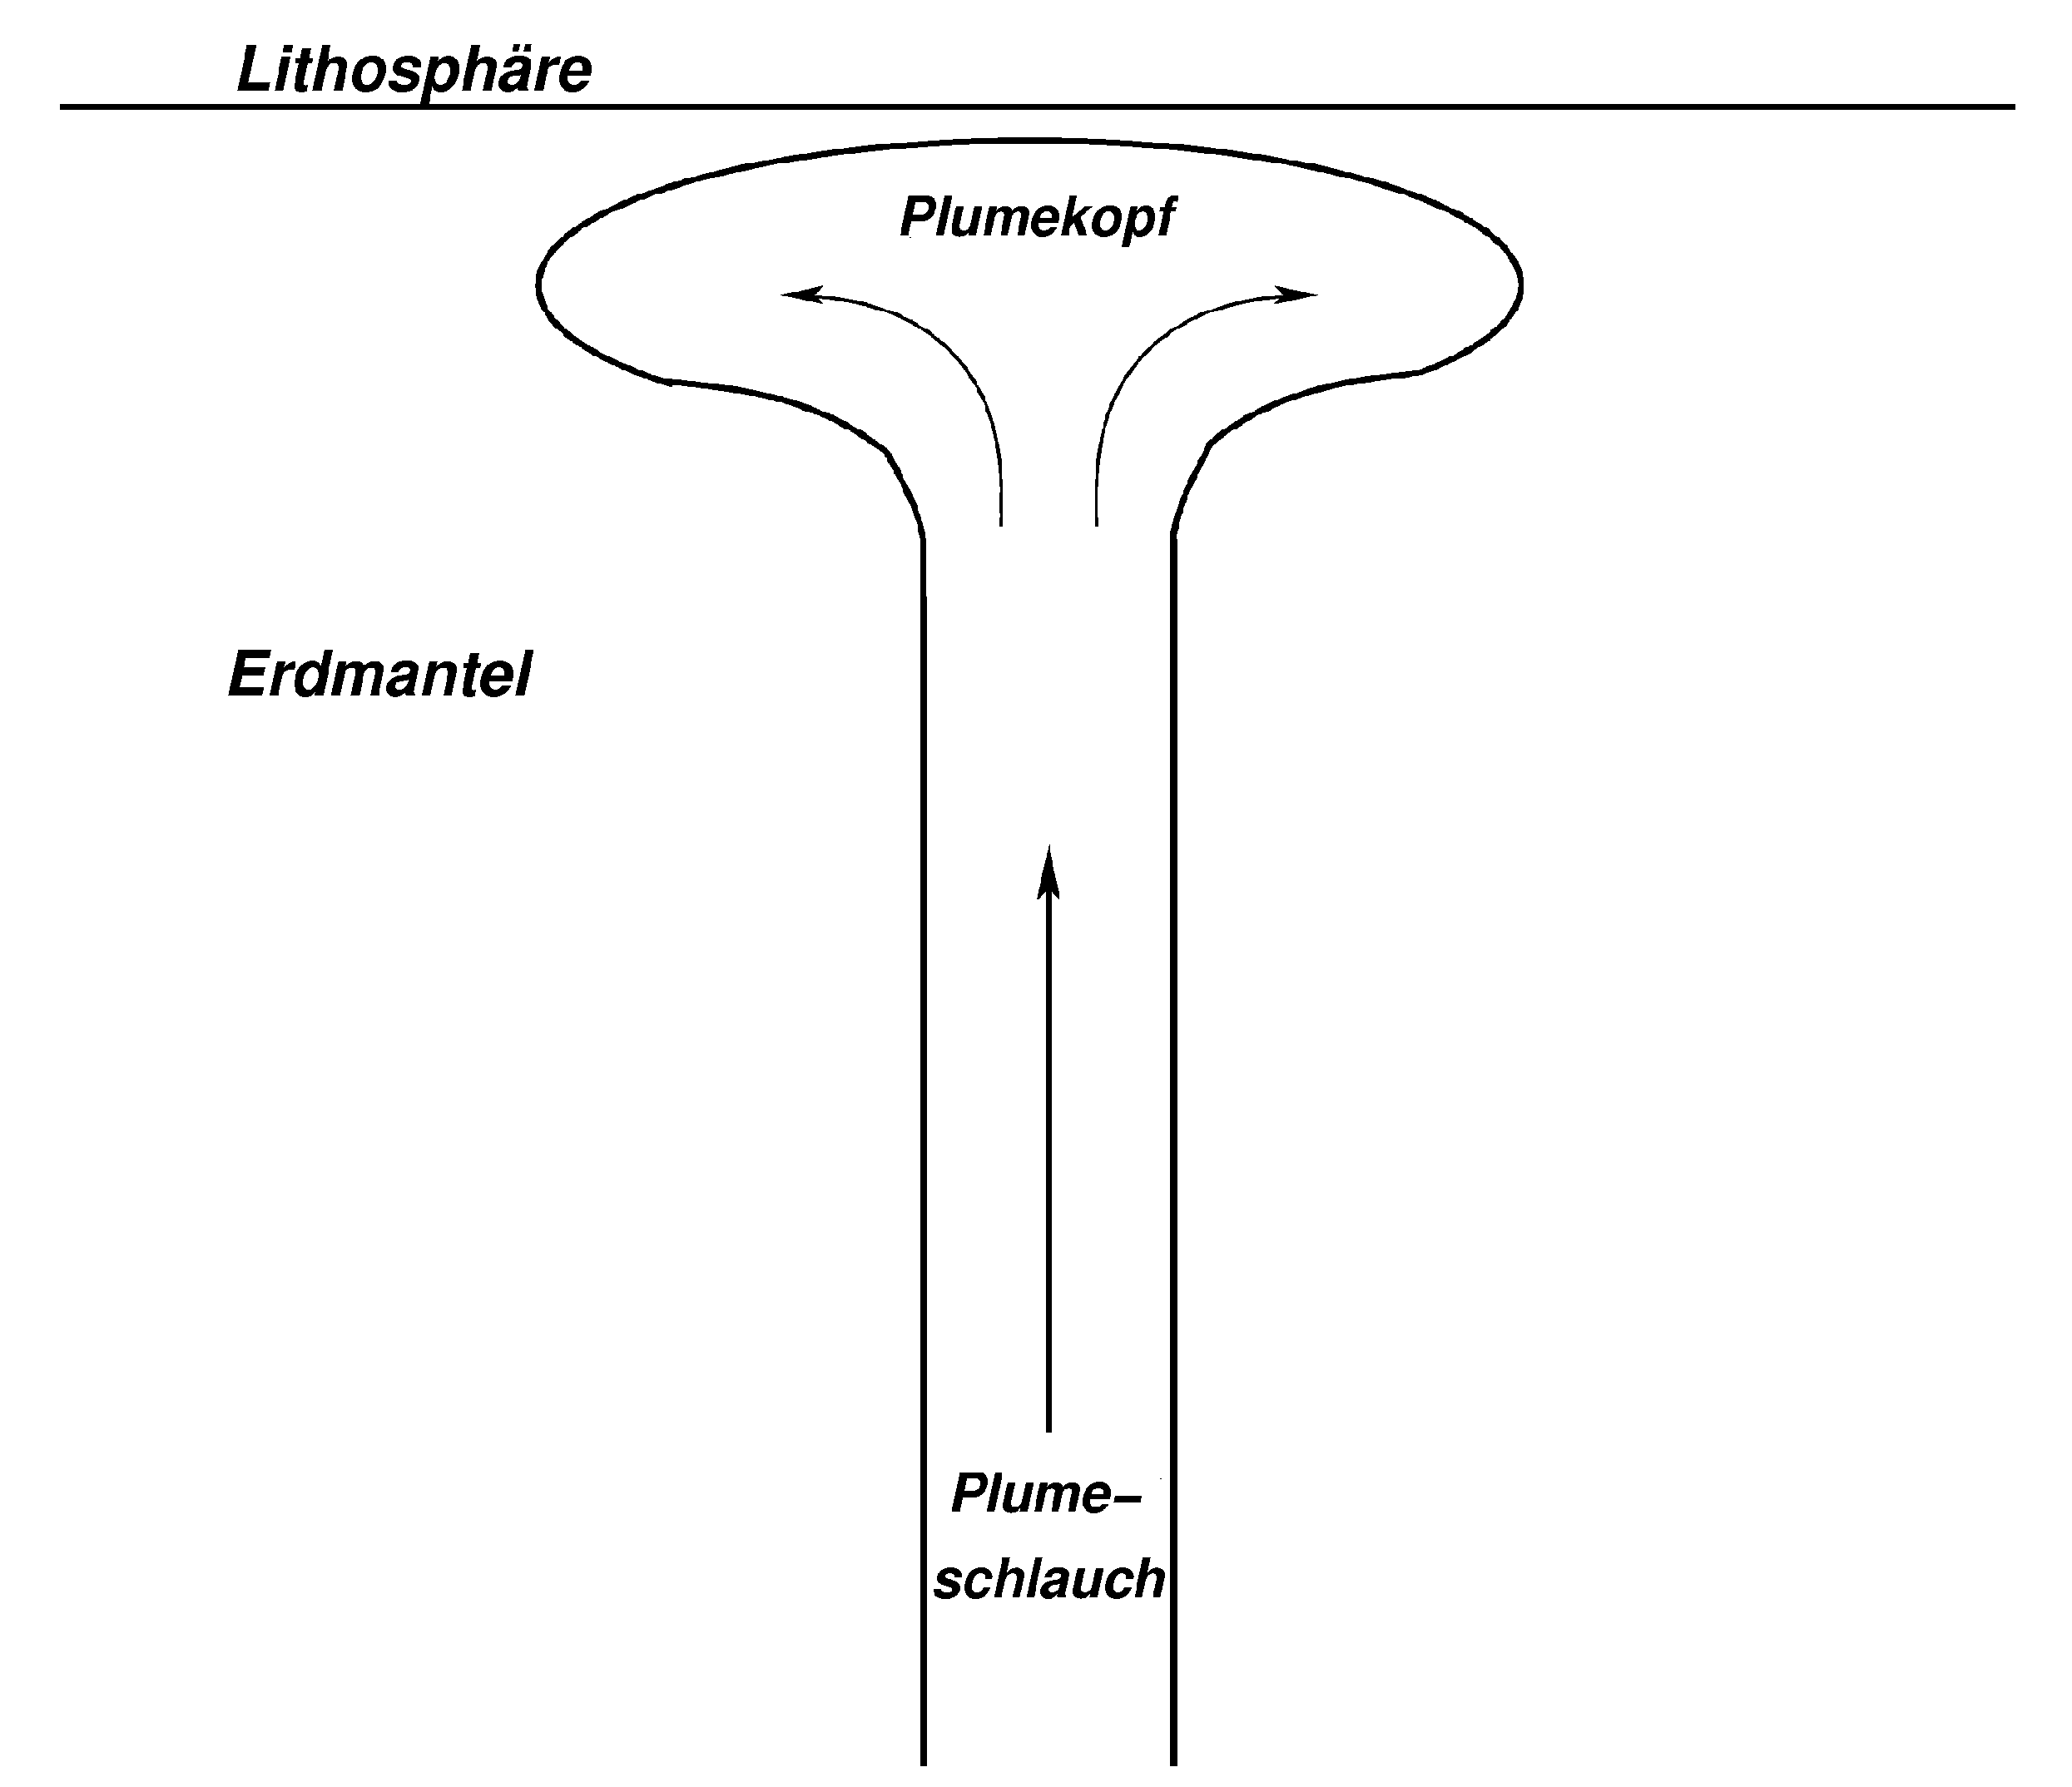
\includegraphics[width=0.5\textwidth]{Plume.png}
\caption{Schema eines Mantelplumes.\protect\footnotemark Der untere Teil des Plumes besteht aus einer auftriebsgetriebenen Aufströmung, welche oben an der Grenze des Mantels eine pilzkopfartige Form annimmt. An dem Ort des Auftreffens steigt die Warscheinlichkeit vukanischer Aktivität.}
\label{fig:plume}
\end{figure}
\footnotetext{\url{https://commons.wikimedia.org/wiki/File:Plume-schematisch.png} vom 05.06.2018 11:30}
Mantelplumes (Plumes im Erdmantel) sind eine Quelle für vulkanische Aktivität.
Häufig gut zu beobachten sind sie an den Schornsteinen von großen Kraftwerken: Man sieht dort häufig kleine „Wolkenstöße“ nacheinander kommen.
Dieses Phänomen kann man auch in Abb. \ref{fig:bromo_plumes} sehen, wo sich die Plumes deutlich in den Abgasen des Vulkans \textit{Mount Bromo} erkennen lassen.
\begin{figure}[!h]
  \centering
  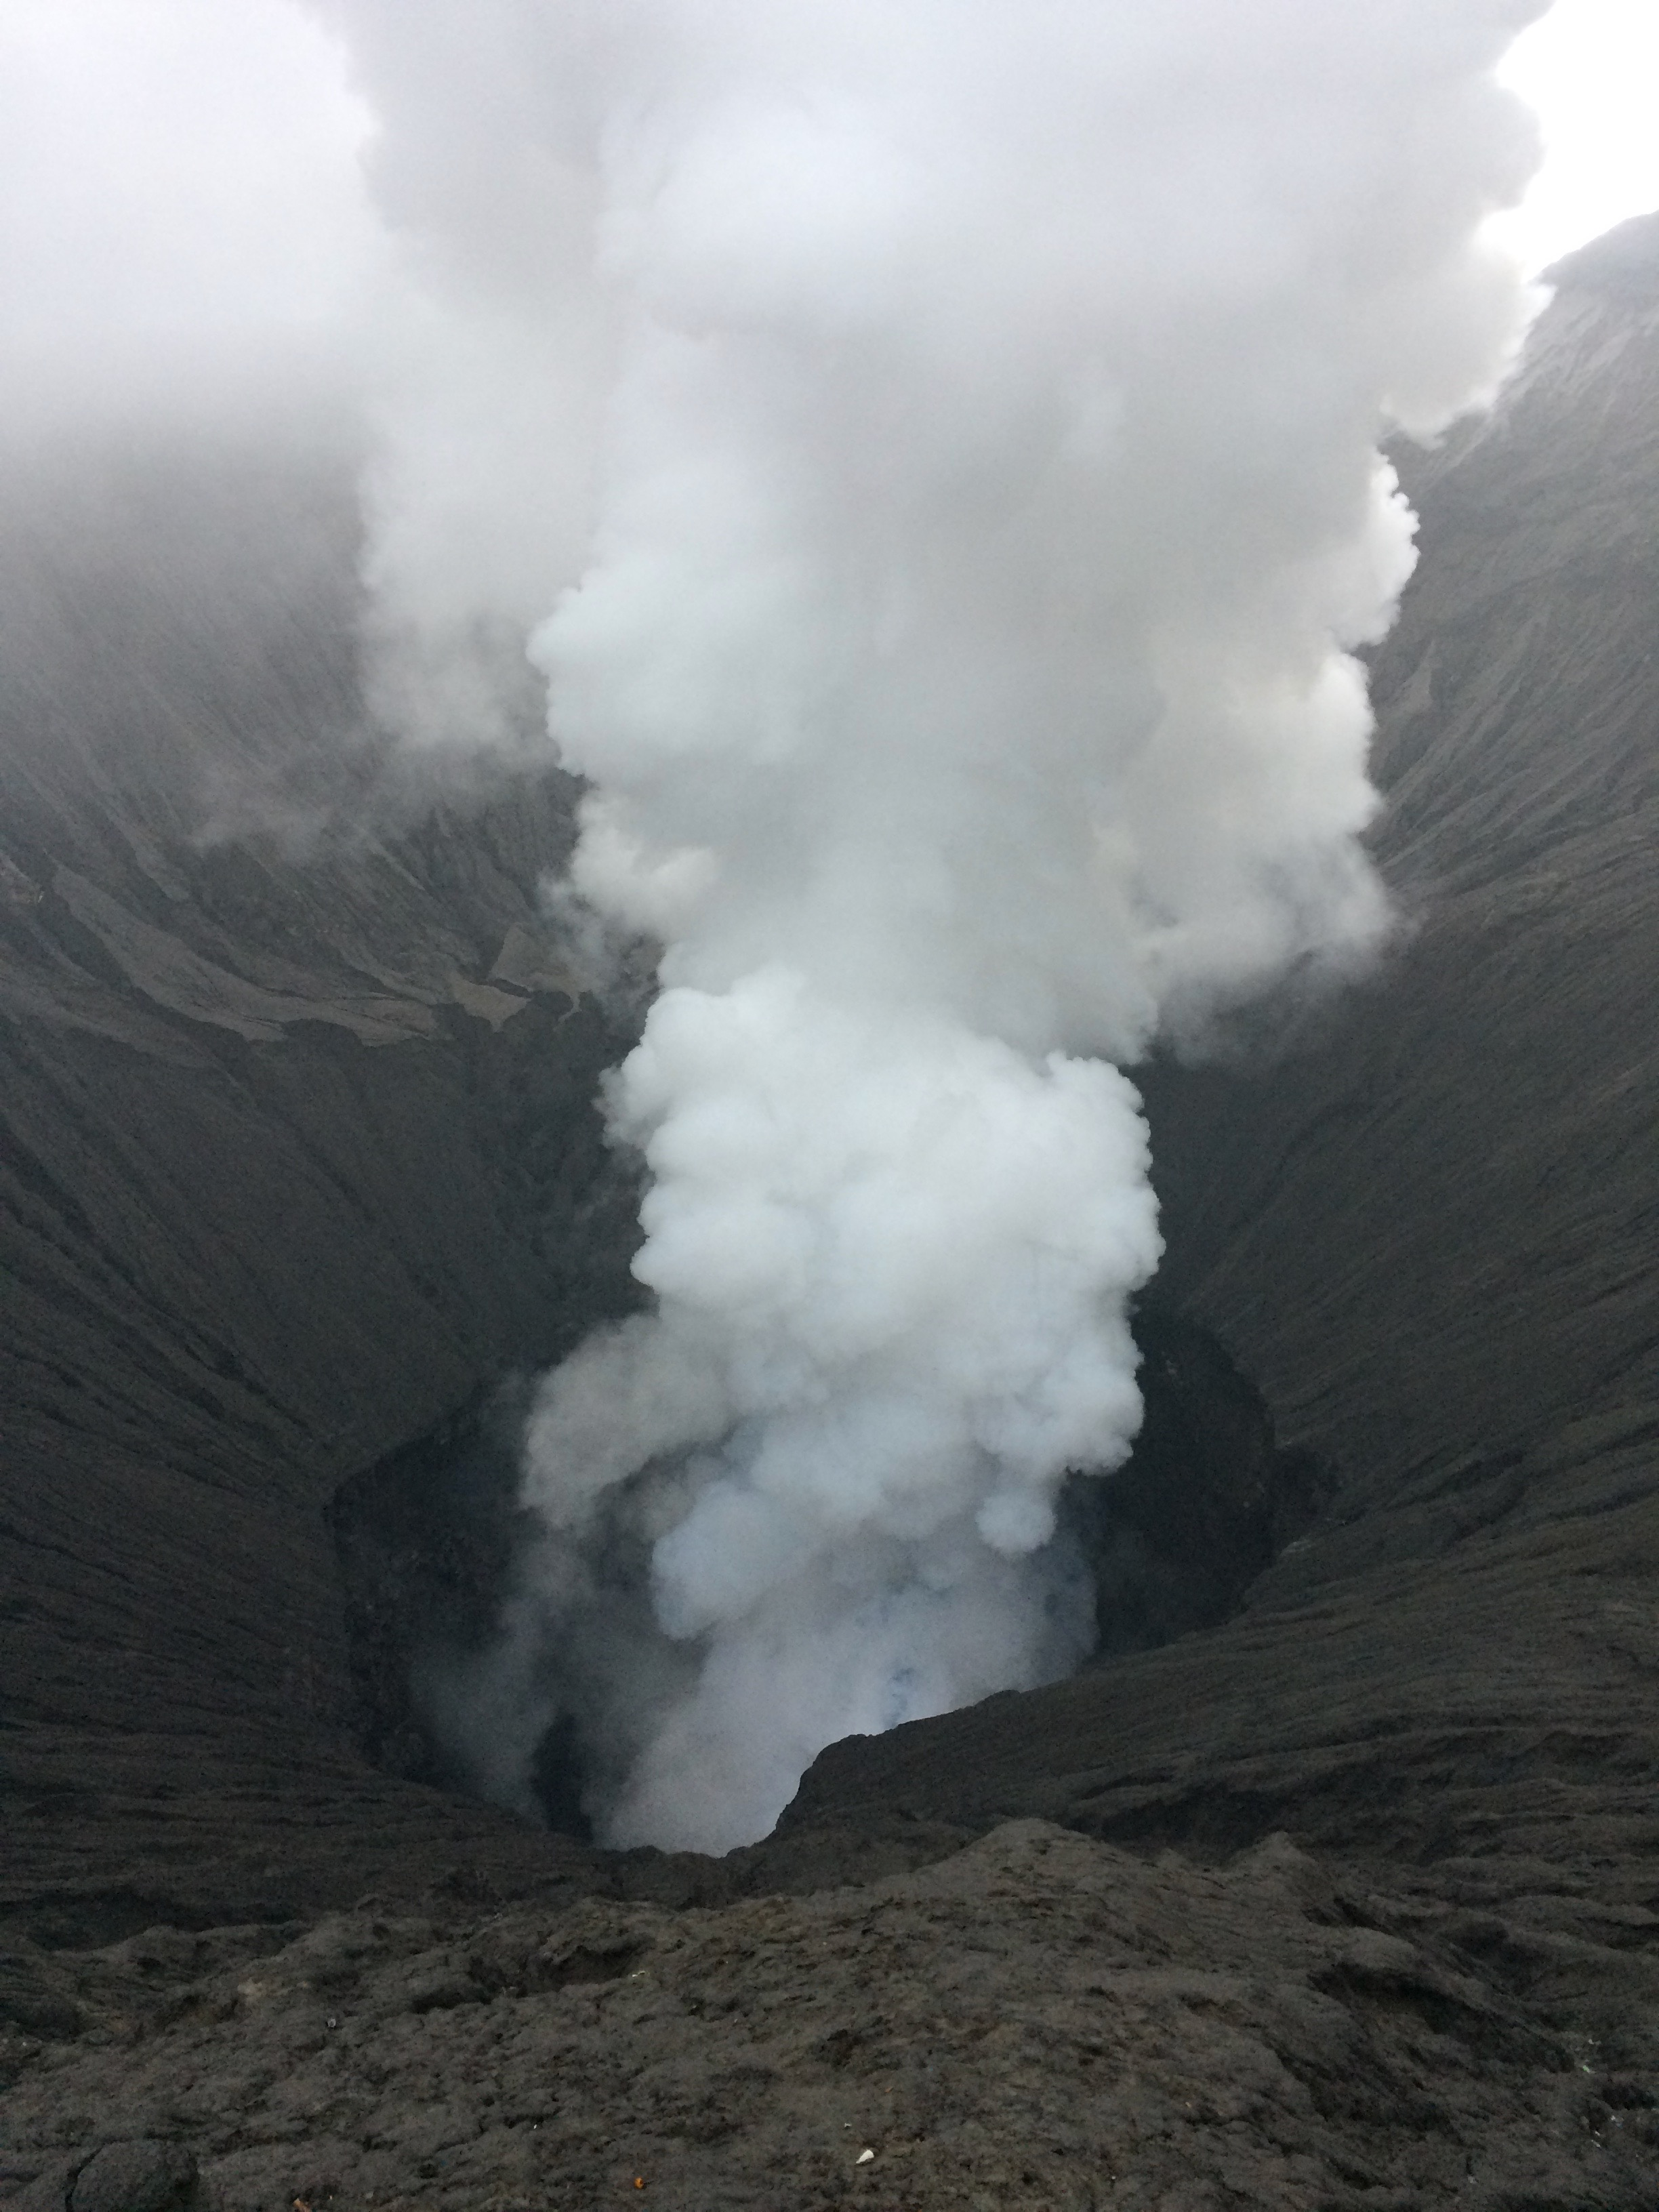
\includegraphics[width=0.4\linewidth]{bromo_plumes}
  \caption{Plumes sichtbar am Beispiel des Mount Bromo (10.1.2017). Gut erkennbar sind die vielen kleinen pilzkopfartigen Dampfbüschel.}
  \label{fig:bromo_plumes}
\end{figure}

\subsection{Large Scale Circulation}
Auf großen Zeit- und Längenskalen dominiert die großräumige Zirkulation (Large Scale Circulation, LSC).
Sie wird durch Reibungseffekte kontinuierlich abgebremst, und durch zeitlich und räumlich statistisch auftretende Plumes im Mittel angetrieben.
Die möglichen Formen der LSC sind sehr vielfältig und können zum Beispiel hexagonal oder auch walzenförmig sein.
Um diese Formen auch in sehr turbulenten Strömungen zu erkennen, muss das Geschwindigkeitsfeld zeitlich gemittelt werden. 
Je kleiner die Rayleigh-Zahl, desto kleiner die Turbulenz und desto kürzer muss der Zeitraum der Mittelung sein, um LCS zu sehen.
\begin{figure}[!ht]
\centering
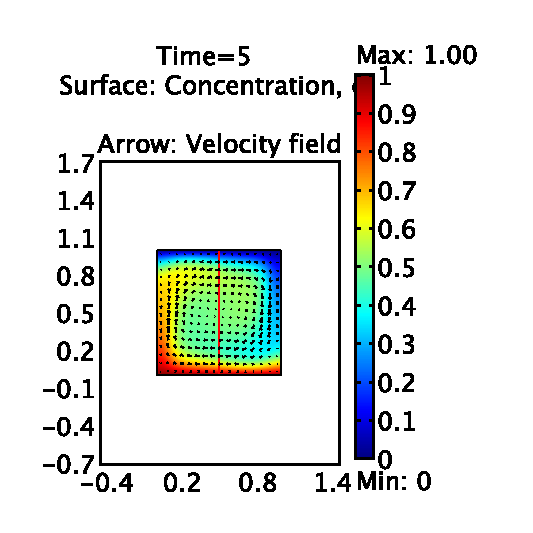
\includegraphics{1e5.eps}
\caption{Ergebnis einer Simulation für $Ra=10^5$. Gut erkennbar ist, dass eine großräumige kreisförmige Strömung existiert, welche an den Rändern und im Zentrum zum erliegen kommt.}
\label{fig:1e5_num}
\end{figure}

Wie häufig ein Plume entsteht und wie stark er (im stochastischen Mittel) eine LSC antreibt hängt von der Rayleigh-Zahl ab und spiegelt sich im Turbulenzgrad wieder.
Diese Plumes sind gut zu messen, da sie einen deutlichen Temperatur- und damit und Dichte-Unterschied zur Umgebung aufweisen.
Hierauf wird in den Kapiteln \ref{sec:schattenproj} und \ref{sec:profile} näher eingegangen.

\newpage
\section{Experiment und Setup}
\label{sec:durchfuehrung}

Die RBK wird in einer kubischen Plexiglas Zelle mit $20\si{\centi\meter}$ vermessen.
Sie wird unten durch eine Metallplatte geheizt und oben gekühlt entsprechen der Randbedingung.
Innerhalb der Zelle befinden sich Thermistoren (s.u.) um die Temperatur zu messen.
Einer ist frei in $z$-Richtung verfahrbar, die anderen sind in festen Abständen aufgereiht.
Erstere dienen zur zeitlichen Korrelation auf-, oder absteigender Strukturen, wie z.B. Plumes.
Letzter wird zur Messung der mittleren Temperatur an bestimmten Orten verwendet.
Ebenfalls sind Thermistoren zu Messung der Plattentemperaturen vorhanden.

Die Widerstände der Thermistoren können durch ein Multimeter oder eine Wheatstonebrücke (ebenfalls s.u.) bestimmt werden.

\subsection{Thermistoren}
Ein Thermistor ist ein temperaturabhängiger Widerstand.
Ist diese Abhängigkeit bekannt, so kann aus dem gemessenen Widerstand die Temperatur zurückgerechnet werden.
Die hier verwendeten Thermistoren sind sogenannte Heißleiter, also Widerstände die mit steigenden Temperaturen geringer werden (NTC-Widerstände).

\subsection{Wheatstonebrücke}
Eine Wheatstonebrücke ist eine Schaltung, bei der durch mehrere bekannte Widerstände und der Messung einer Spannung ein Widerstand bestimmt werden kann.
Ein Schaltplan kann in der Abbildung \ref{fig:wheat} eingesehen werden.
\begin{figure}[!ht]
\centering
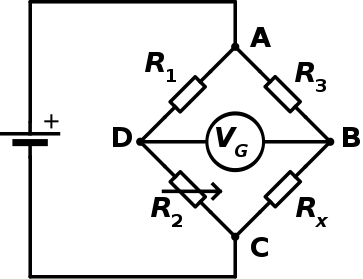
\includegraphics[width=0.5\textwidth]{Wheatstone.png}
\caption{Schaltung einer Wheatstonebrücke.\protect\footnotemark}
\label{fig:wheat}
\end{figure}
\footnotetext{\url{https://commons.wikimedia.org/wiki/File:Wheatstonebridge.svg} vom 01.06.2018 10:40}

Die Widerstände $R_1$ und $R_3$ sind bekannt.
Das Potentiometer $R_2$ wird zur Eichung der Brücke verwendet und der unbekannte Widerstand $R_x=R_{th}$ ist der Thermistor.
Ist die Brücke abgeglichen, sprich die Spannung $V_G=0$, so kann man unter Zuhilfe der Kirchhoffschen Knoten- und Maschen-Regeln nachrechnen, dass gilt
\begin{align*}
	\frac{R_3}{R_1}=\frac{R_x}{R_2}\quad.
\end{align*}

Ändert sich der Widerstand $R_1\rightarrow R_1+\Delta R$, so kann durch Nachrechnen der Kirchhoffschen Knoten- und Maschenregel folgende Identität für das Spannungsverhältnis hergeleitet werden:
\begin{align}
	\frac{U_5}{U}=\frac{1+v}{1+v+k}-\frac{1}{1+k}\quad.
	\label{eq:spannungsveraeltnis}
\end{align}
Dabei bezeichnet $v=\frac{\Delta R_1}{R_1}$ die Verstimmung und $k=\frac{R_2}{R_1}=\frac{R_x}{R_3}$ das Brückenverhältnis.

\subsection{Nyquist-Shannon-Abtasttheorem}
Das \textsc{Nyquist-Shannon}-Abtasttheorem besagt, dass man zur korrekten Rekonstruktion eines Signals $S$ dieses mit mehr als der doppelten maximal darin vorkommenden Frequenz $f_{\text{max, }S}$ messen muss.
Andernfalls kann es zu sogenannten „Sampling-Effekten“ kommen, bei denen das Rekonstruierte Signal eine deutlich geringere Frequenz aufweist, als das tatsächliche.
Dieses ist in Grafik \ref{fig:nyquist} gut zu erkennen.
\begin{figure}[h]
  \centering
  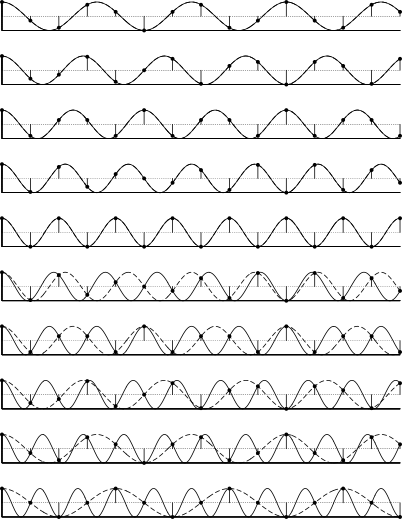
\includegraphics[width=0.4\linewidth]{nyquist}
  \caption{Beispiel, weshalb eine geringere Messfrequenz als $2f_{\text{max, }S}$ nicht ausreichend ist.\protect\footnotemark\label{fig:nyquist}}
\end{figure}
\footnotetext{\url{https://commons.wikimedia.org/wiki/File:Nyquist_Aliasing.svg} vom 17.06.2018 14:45}

\subsection{Spektrum einer Zeitserie und Korrelation}
Das Spektrum eines Signales beschreibt, welche Frequenzen in ihm vorkommen.
Nimmt man eine Zeitserie der Temperatur an einem Ort auf, so entspricht das fouriertransformierte Signal den Frequenzen mit der Temperaturschwankungen auftreten.
Diese kommen durch Plumes zustande.

Möchte man nun deren Geschwindigkeit messen, so bietet es sich an, eine Thermistor-Kette zu nehmen und mit ihr eine Langzeitmessung zu machen.
Korreliert man die Daten benachbarter Thermistoren miteinander, so kann man mittels ihres Abstandes und des Maximums in der Korrelation die mittlere Geschwindigkeit der Plumes feststellen.
Natürlich gibt es keine perfekte Korrelation, da sich die Form der Plumes während des Aufsteigens verändert.
Sie berechnet sich aus der Faltung der beiden Signale:
\begin{align}
	(f*g)(t)=\int f(\tau)g(t-\tau) d\tau\quad.
	\label{eq:faltung}
\end{align}
Das Maximum in der Kurve gibt nun an, mit welche Abstand die meisten Plumes an den beiden Thermistoren vorbeikamen.
Da das Ausrechnen des Integrals für alle Zeiten $t$ sehr rechenintensiv ist, kann man stattdessen vom \textit{Faltungstheorem} gebrauch machen, welches besagt
\begin{align}
	\mathcal F(f*g)=\sqrt{2\pi}\mathcal F(f)\cdot\mathcal F(g)\quad.
	\label{eq:faltungssatz}
\end{align}
Dadurch muss man nur noch das Produkt der Fouriertransformierten ausrechnen und das Ergebnis rücktransformieren.


\newpage
\section{Ergebnisse}
\label{sec:auswertung}

\subsection{Schattenprojektion}
\label{sec:schattenproj}
Bei einer Schattenprojektion wird ein Fluid mittels einer hellen Lampe angestrahlt und hinter dem Fluid wird ein Schirm beobachtet.
Durch diesen Aufbau sind Dichteunterschiede erkennbar, da sie in Brechungsindex-Variationen resultieren, welche dann zu helleren bzw. dunkleren Regionen auf dem Schirm führen.
Um die Geschwindigkeit der Plumes zu bestimmen wird die Bewegung ihrer Schatten auf einem Schirm beobachtet und die Laufzeit durch bestimmte Abstände gemessen.
Die gemessene Lauflänge der Schatten auf den Schirm muss noch mithilfe des Strahlensatzes umgerechnet werden um die korrekte Strecke, welche die Plumes tatsächlich durchlaufen haben, zu erhalten.\\

Um die Position der Plumes in der Zelle genauer bestimmen zu können wird orthogonal zur ersten Richtung ein zweites Mal gemessen.
Dadurch lässt sich ermitteln, in welchem Quadranten die Plumes auf und absteigen.
%Skizze der von uns gemessenen Quadranten
\\
%Tabelle der Daten mit Fehlern und Raynolds Zahl



\subsection{Wahl der Messfrequenz}

\begin{figure}[!ht]
\centering
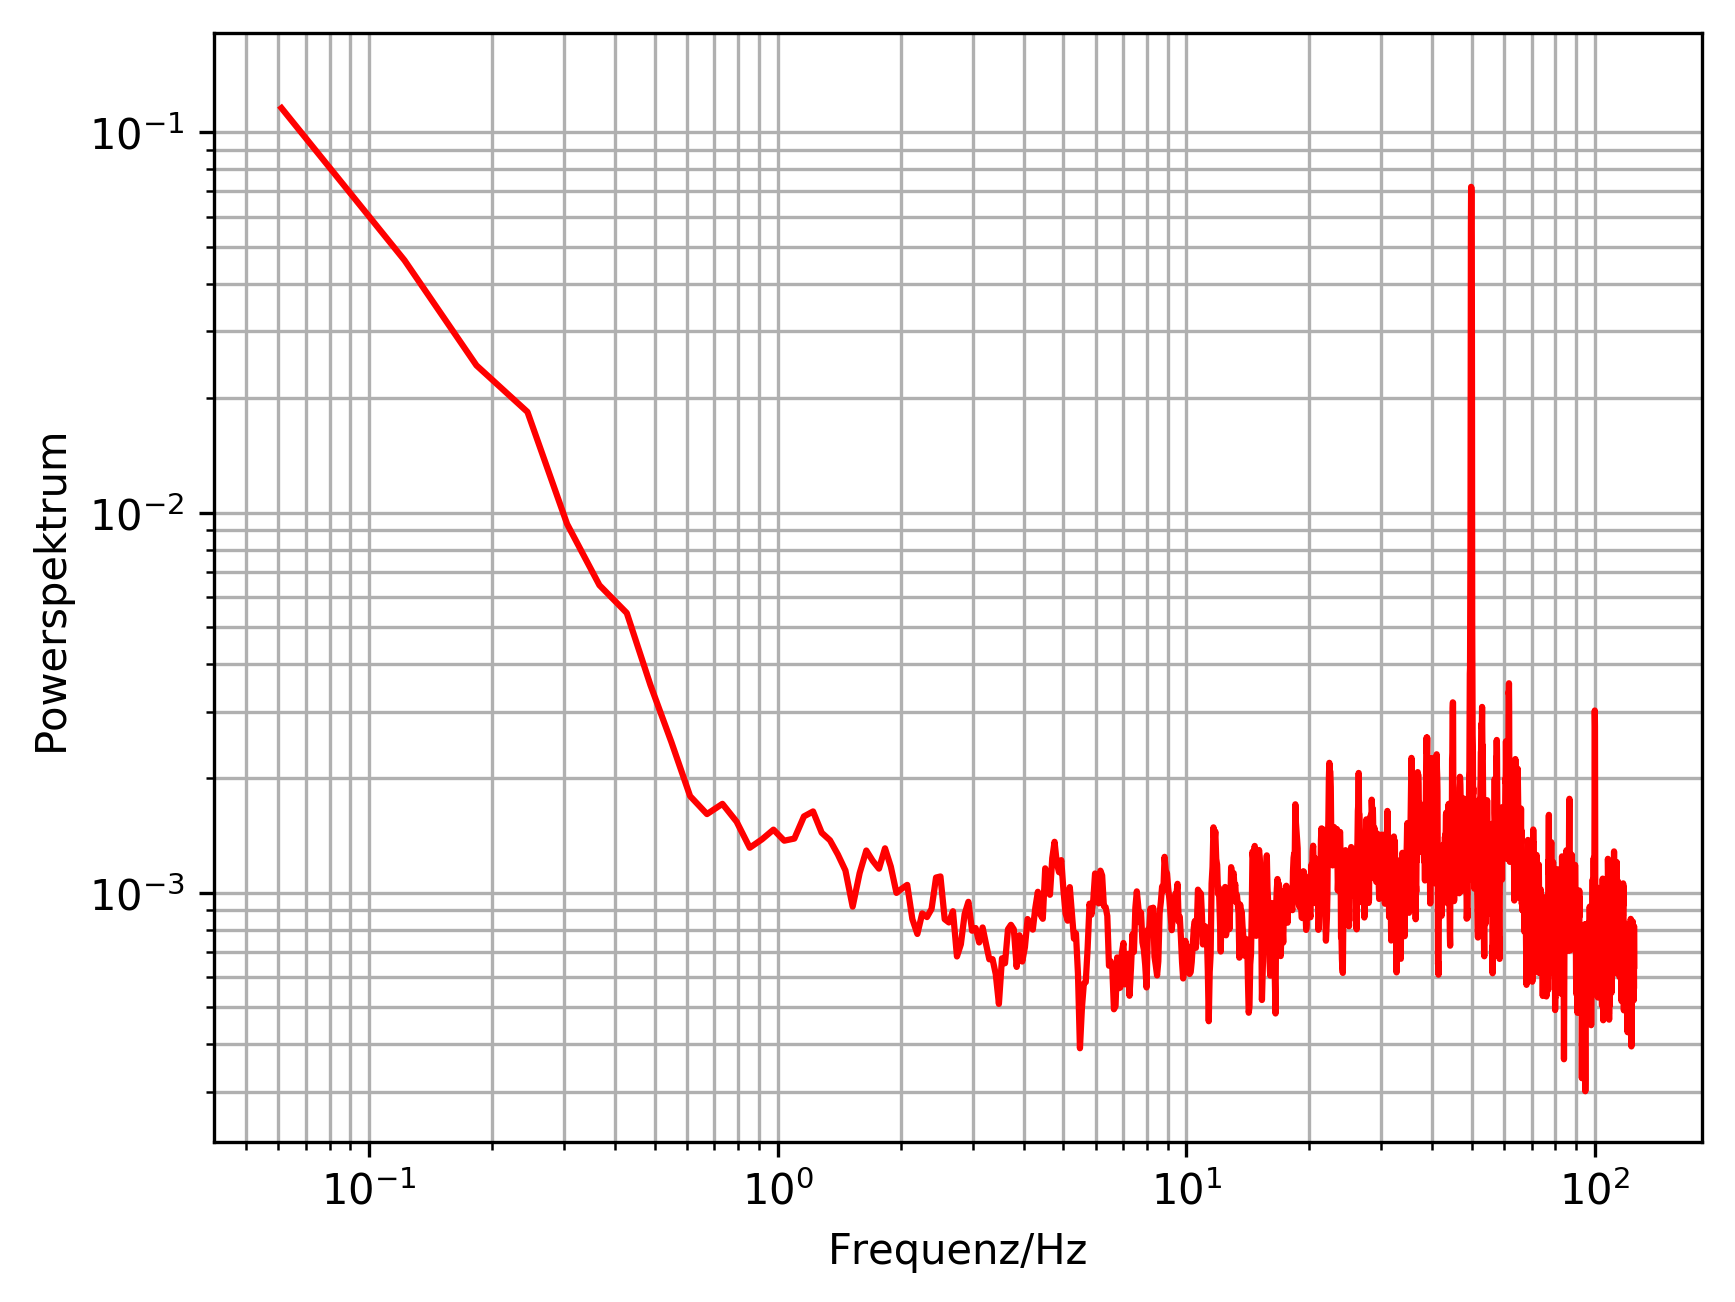
\includegraphics[width=0.8\textwidth]{stoer.png}
\caption{Spektrum der Störfrequenz-Messung in der Mitte der Zelle mit einer Messfrequenz von $250\si{\hertz}$. Die größte Störfrequenz von $50\si{\hertz}$, welche der Netzspannungsfrequenz entspricht, ist klar erkennbar.}
\label{fig:stoer}
\end{figure}

Da jede Messung natürlich externe Störsignale beeinflusst wird, maßen wir einige Minuten im Zentrum der Zelle mit $\SI{250}\hertz$.
In Abb. \ref{fig:stoer} sind die gemessenen Frequenzen aufgetragen.
Deutlich zu erkennen ist die Netzfrequenz bei $50\si{\hertz}$.
Desweiteren sind auch die harmonischen (vielfachen) dieser Frequenz zu erkennen, allerdings am besten bei $200\si{\hertz}$.\\
Unterhalb von etwa $10\si{\hertz}$ ist starkes Rauschen im zeitlichen Signal sichtbar.
Zudem sind einige kleinere weitere Linien im Spektrum erkennbar, welche beispielsweise von den internen Frequenzen der umliegenden Geräten stammen könnten.

Das Aliasing ist ein Effekt, der nach dem Shannon-Nyquist-Abtasttheorem zustande kommt, wenn die zu messende Frequenz nicht mit mehr als der doppelten Frequenz gesamplet wird.
Dann kann es dazu kommen, dass eine hohe Frequenz durch Samplen in verschiedenen Zyklen im Signal von einer viel geringeren Frequenz ununterscheidbar ist.
Um dies zu unterdrücken muss eine Messfrequenz $f_s$ bestimmt werden bei der diese Störfrequenzern durch den Aliasing Effekt nicht übermäßig im verwendeten Teil des Spektrums auftreten.
Die sogenannte \textit{Aliasing Frequenz} $f_a$, welche der gemessenen Frequenz eines eigentlich wesentlich höherfrequenten Signals $f$ entspricht, berechnet sich aus
\begin{align}
  f_a=|f-n\cdot f_s|\quad,
  \label{eq:stoerfreq}
\end{align}
da negative Frequenzen durch die Symmetrie des Kosinus auch auf die positive Achse gespiegelt werden können (oder anders: es kommt nur auf die absolute Differenz der Signale an)

Will man nun den Einfluss der Störfrequenzen in dem gemessenen Signal minimieren, so muss man die Messfrequenz so wählen, dass
\begin{align}
  \sum_{f_\text{ref}} |I(f)-I(f_\text{ref})|
\end{align}
minimal wird.

Bei uns war dies bei etwa $\SI{9.1}\hertz$ der Fall, so dass die folgenden Messungen mit ebendieser Frequenz aufgenommen wurden.

\subsection{Geschwindigkeits- und Temperaturprofil}
\label{sec:profile}
In Grafik \ref{fig:T_fahrt} ist das höhenabhängige Temperaturprofil im Zentrum der Zelle aufgetragen.
Dabei stellt die rote Kurve den Mittelwert dar und der blaue Bereich zeigt die zeitliche Standardabweichung an.
Deutlich zu erkennen ist die Grenzschicht an der unteren Heizplatte.
In ihr ist auch die Standardabweichung gering, was darauf schließen lässt, dass das Fluid dort kaum turbulent ist und so thermisch stabil (was aufgrund der Theorie auch so zu erwarten ist).
\begin{figure}[!ht]
\centering
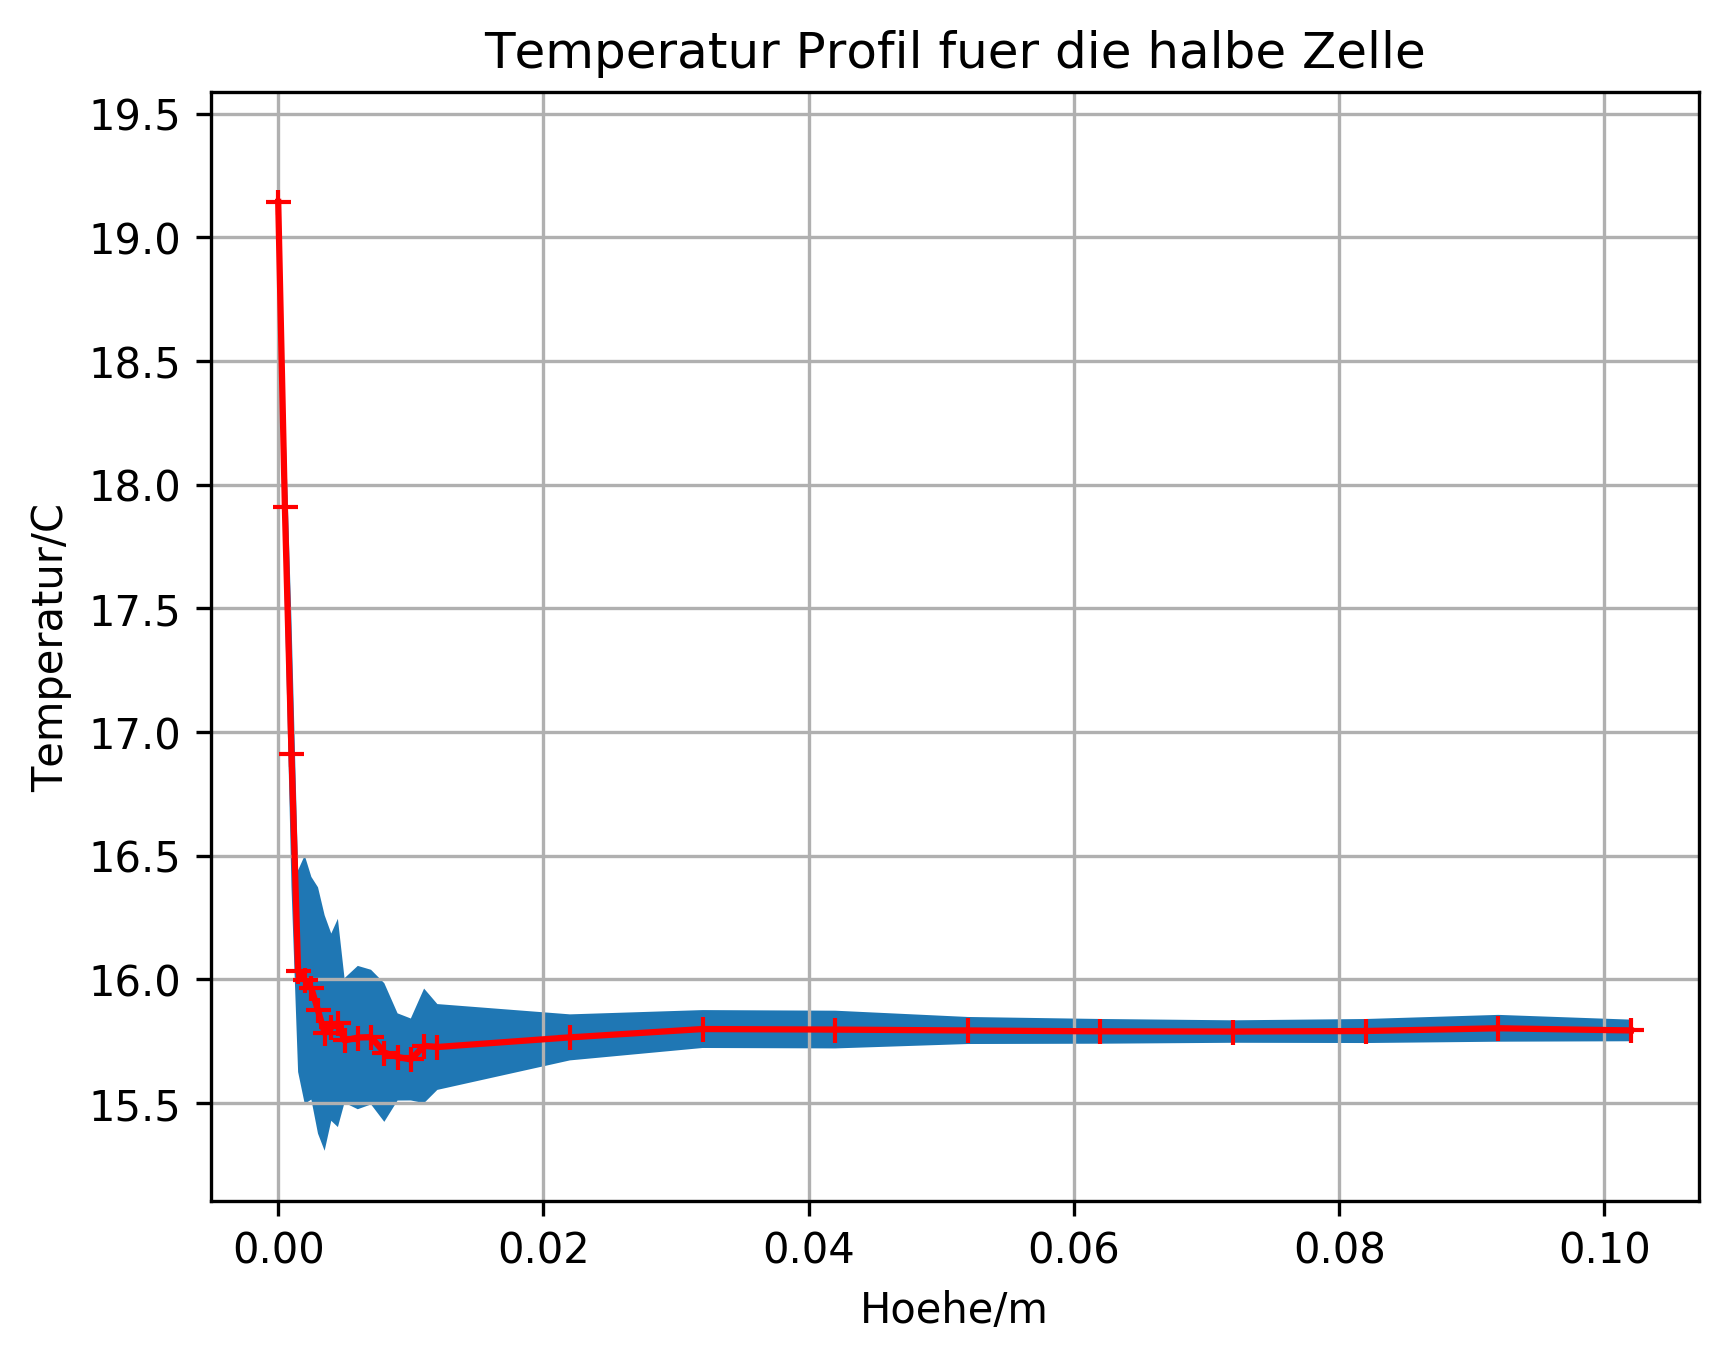
\includegraphics[width=0.8\textwidth]{T_fahrt.png}
\caption{Gemessenes Temperaturprofil}
\label{fig:T_fahrt}
\end{figure}


\subsection{Simulierte Profile und Daten}
Da die Konstruktion und Durchführung von Experimenten mit unterschiedlichen Rayleigh-Zahlen aufwändig ist, greifen Experimentatoren in diesem Bereich gerne auf Simulationen zurück.
Allerdings steigt der Rechenaufwand für große Rayleigh-Zahlen rasant an, so dass es irgendwann nicht mehr sinnvoll ist.
Auch sind die hier durchgeführten Simulationen nur zweidimensional, wodurch bestimmte Effekte des Experiments nicht rekonstruiert werden können.
Dennoch stimmen die Ergebnisse im Allgemeinen gut mit den Messwerten überein.\\

In Abb. \ref{fig:v_num} <++++++++++++++++++++++++++++++++++++++++++++++++++++++++++++++++++++++++++++++++>
\begin{figure}[!ht]
	\centering
    \begin{subfigure}[t]{0.49\textwidth}
        \centering
	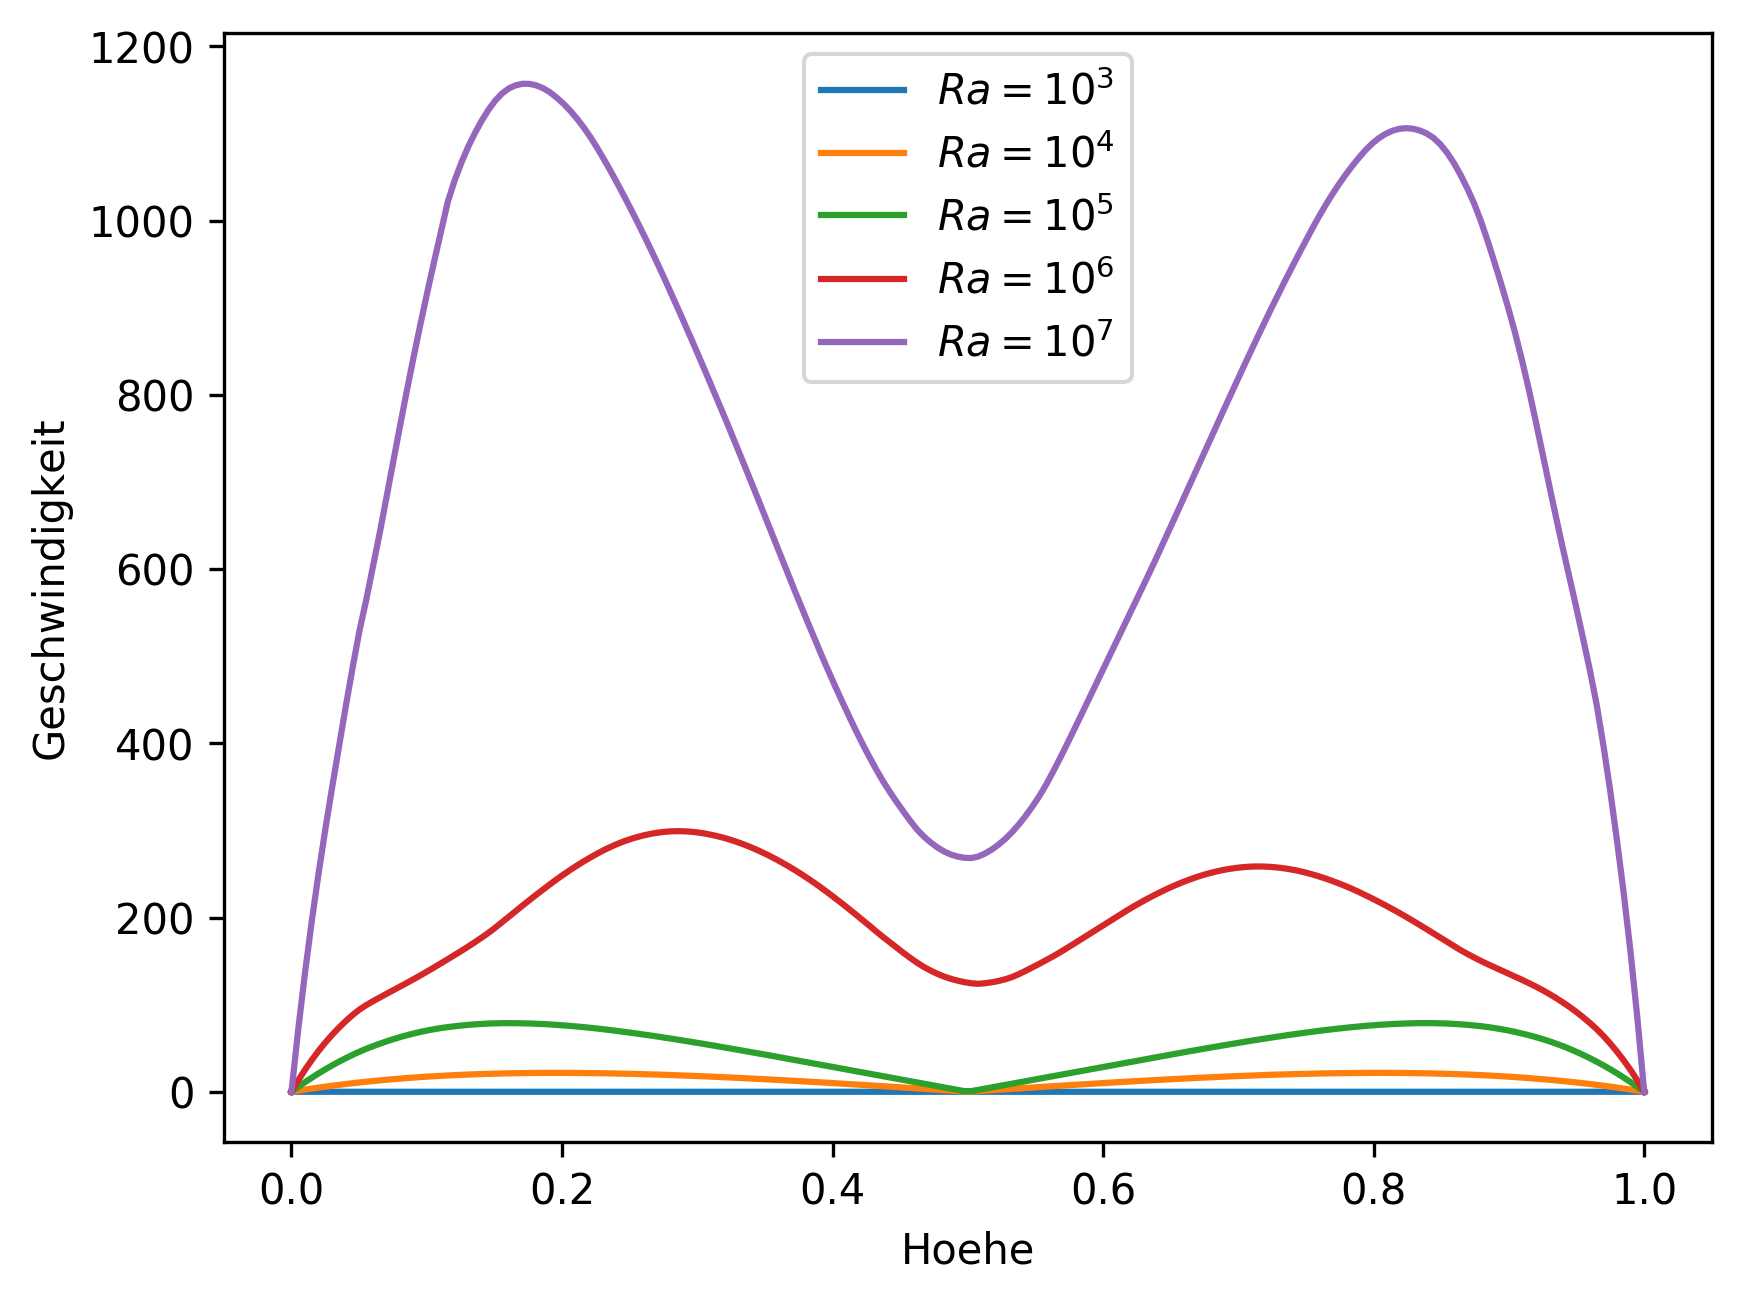
\includegraphics[width=0.9\linewidth]{V}
        \caption{Geschwindigkeitsprofil}
	\label{fig:v_num}
    \end{subfigure}%
    ~ 
    \begin{subfigure}[t]{0.49\textwidth}
        \centering
	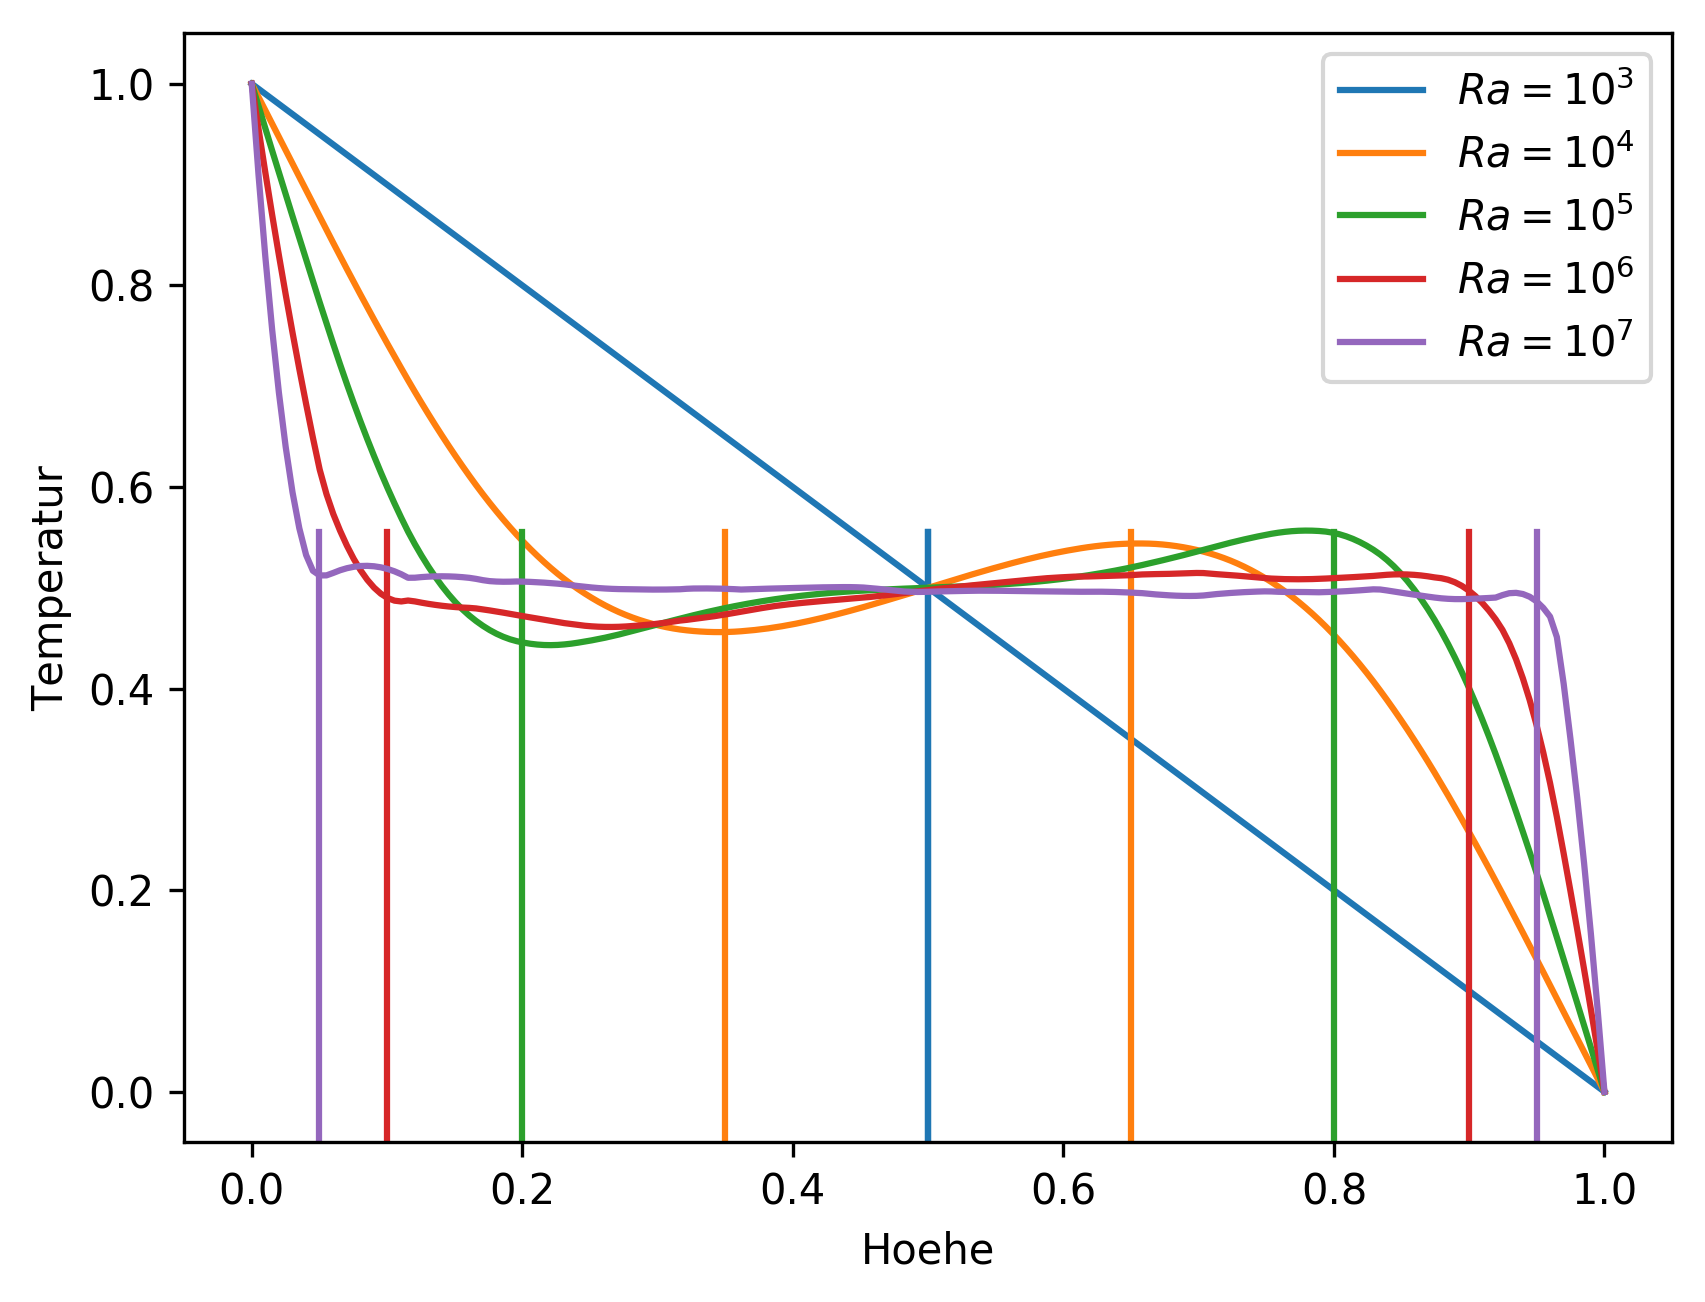
\includegraphics[width=0.9\linewidth]{T}
        \caption{Temperaturprofil}
	\label{fig:t_num}
    \end{subfigure}
    \caption{Simulationen für verschiedene Rayleigh-Zahlen.}
\end{figure}

\begin{figure}[!ht]
\centering
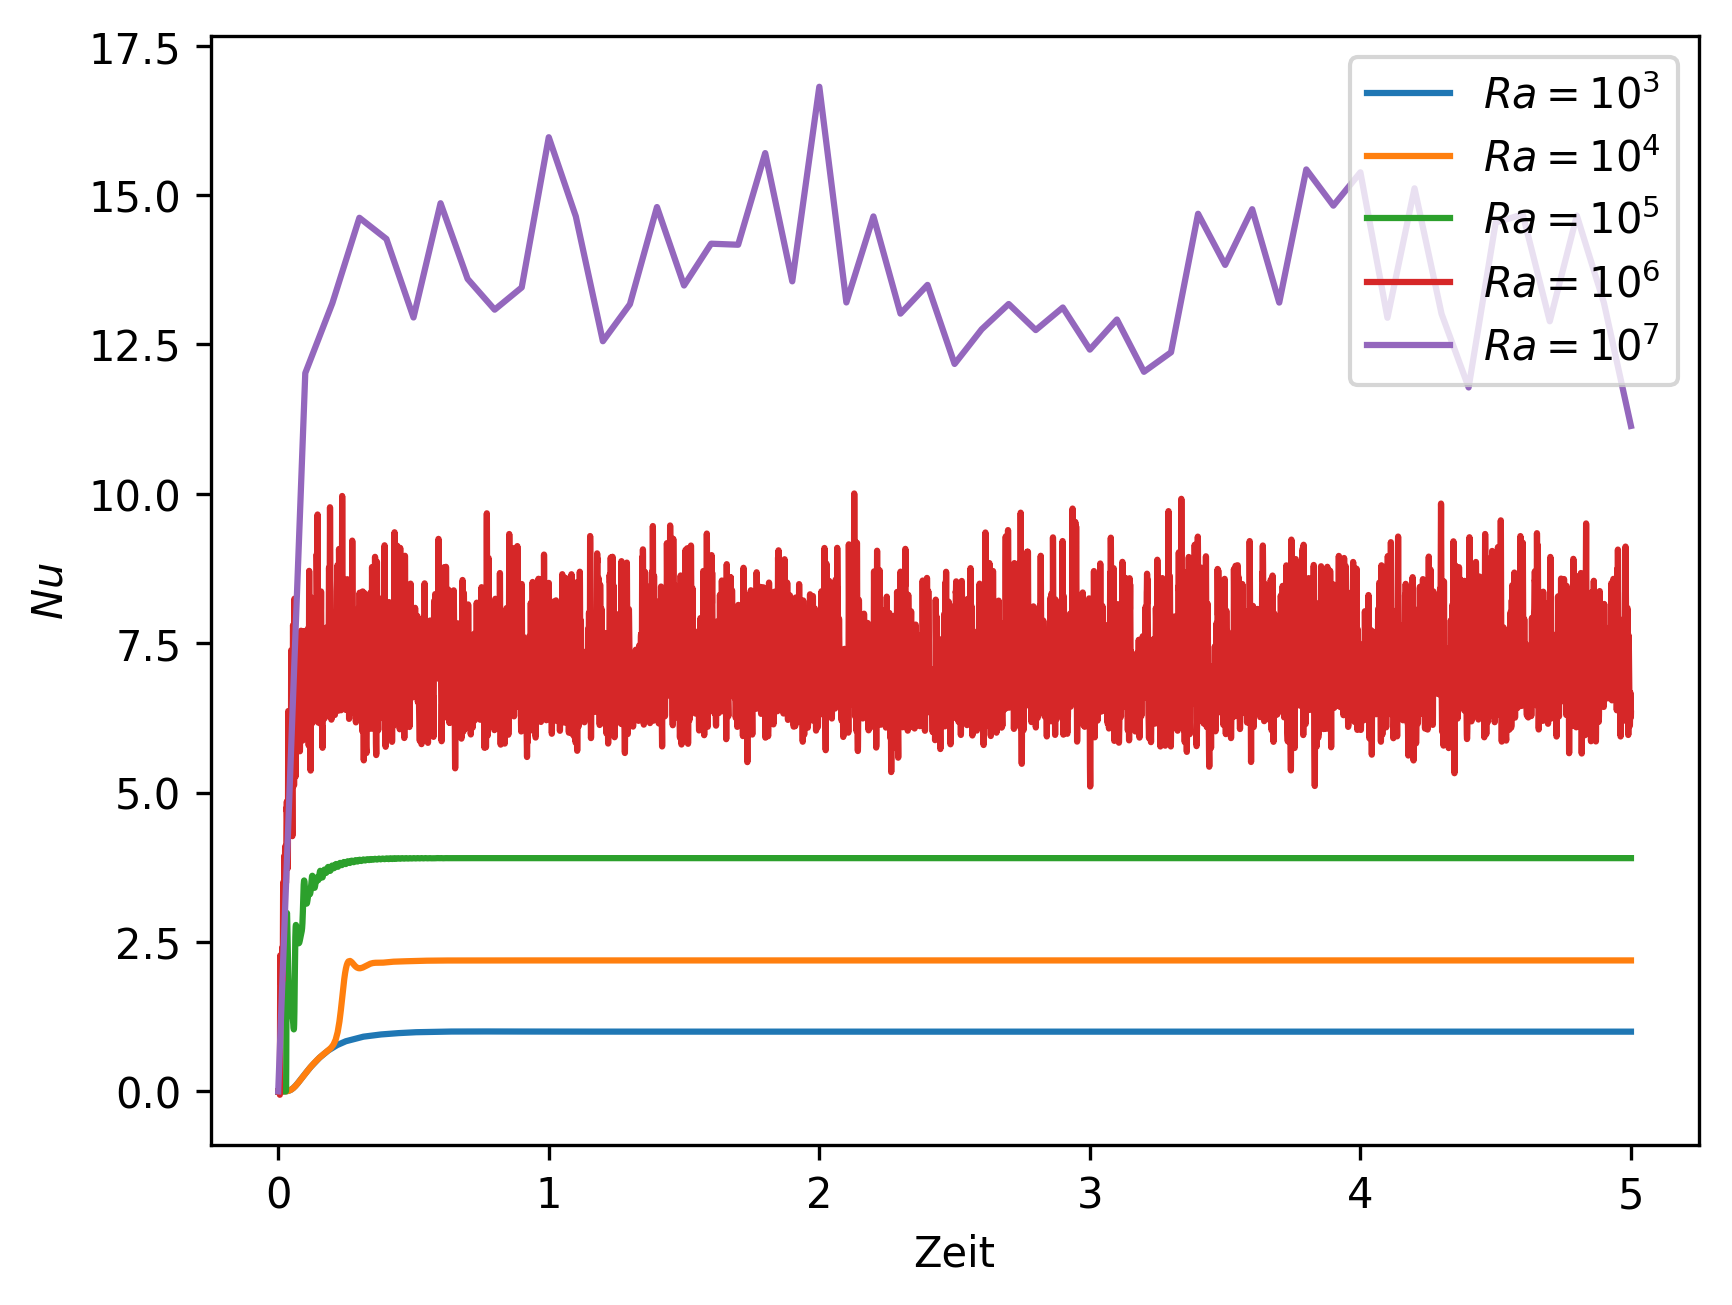
\includegraphics[width=0.8\textwidth]{Nu.png}
\caption{Nusselt Zahl}
\label{fig:nu_num}
\end{figure}





\subsection{Langzeit- und Korrelationsmessung}
In Abbildung \ref{fig:korrelation} ist die Korrelation zwischen aufeinanderfolgenden Thermistoren aufgetragen.
Zu erkennen ist deutlich, dass die Maxima nicht an der selben Position sind.
Dies ist auch in Figure \ref{fig:V_kor} zu erkennen, in der die Geschwindigkeiten (basierend auf der Peak-Position) aufgetragen sind.
Dabei ist zu beachten, dass die Thermistoren nicht äquidistant sind.\\

Die Breite der Korrelation kann man nicht ohne weiteres auswerten, da dort noch zahlreiche Effekte herein spielen, wie die Entstehung eines Plumes beeinflusst die Bildung eines weiteren und noch wichtiger: ein Plume bildet in den Messdaten keinen $\delta$-Peak, sondern er ist in der Größenordnung des Abstands der Thermistoren.
Dadurch verschwindet die Korrelation nicht bei $t=0$ und die Breite des Peaks ist nicht nur durch die Geschwindigkeitsverteilung unterschiedlicher Plumes beeinflusst.

\begin{figure}[!ht]
	\centering
	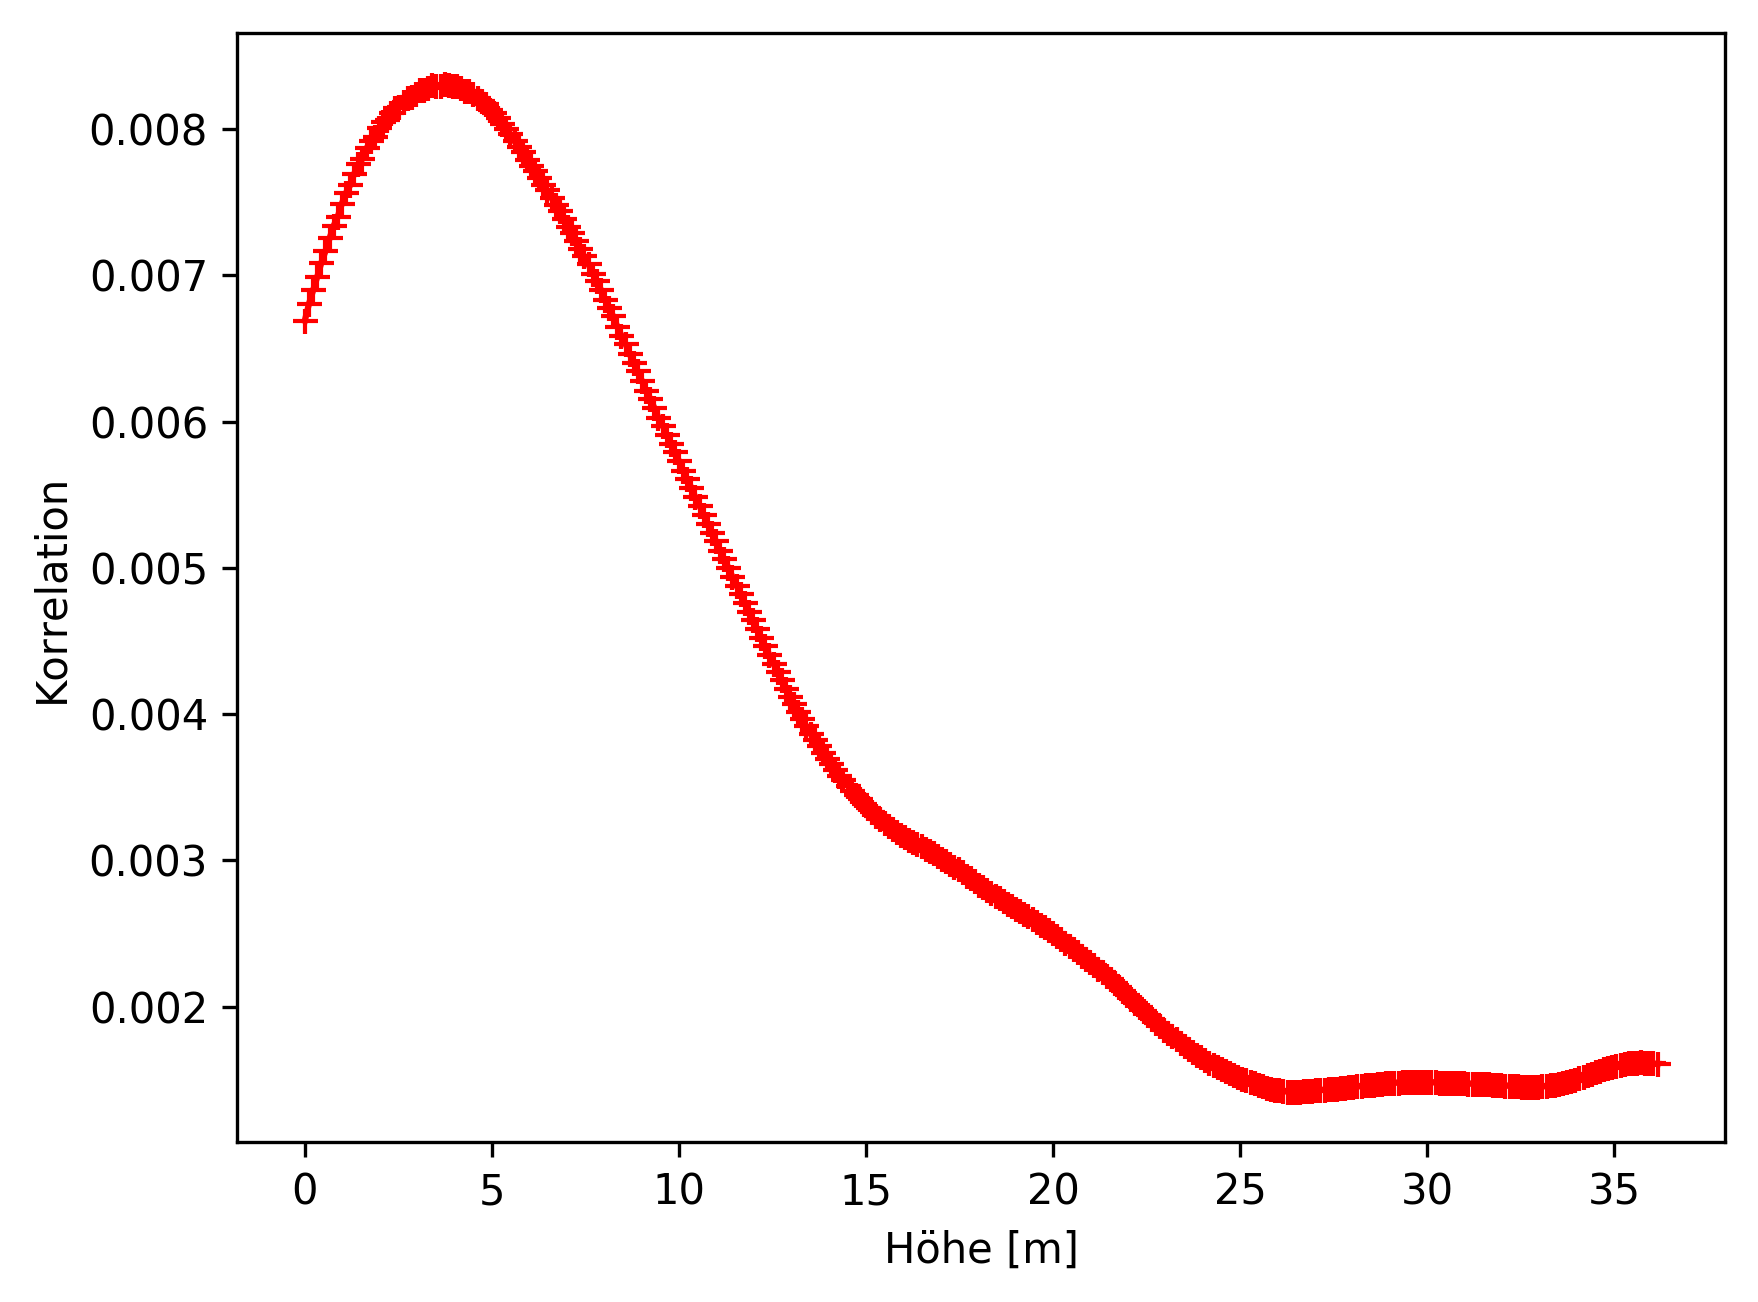
\includegraphics[width=0.7\linewidth]{kor}
	\caption{Korrelation zwischen den Signalen aufeinanderfolgender Thermistoren. Die Maxima befinden sich zwischen $3.7$ und $6.2\si\s$.}
\label{fig:korrelation}
\end{figure}


Aus der Langzeitmessung kann man jedoch die Temperaturdaten für die einzelnen Höhen nutzen, um diese miteinander im Mittelwert zu vergleichen.
Selbiges ist in Grafik \ref{fig:T_kor} aufgetragen.
Zu sehen ist, dass die Standardabweichung sehr viel größer ist, als die Schwankungen der Mittelwerte in verschiedenen Höhen.
Dies steht im Einklang mit der Theorie, da die Wärme ja im Inneren des Containers konvektiv an allen Thermistoren vorbeigeleitet wird, ohne dabei nennenswert Energie zu verlieren oder zu gewinnen.
\begin{figure}[!ht]
\centering
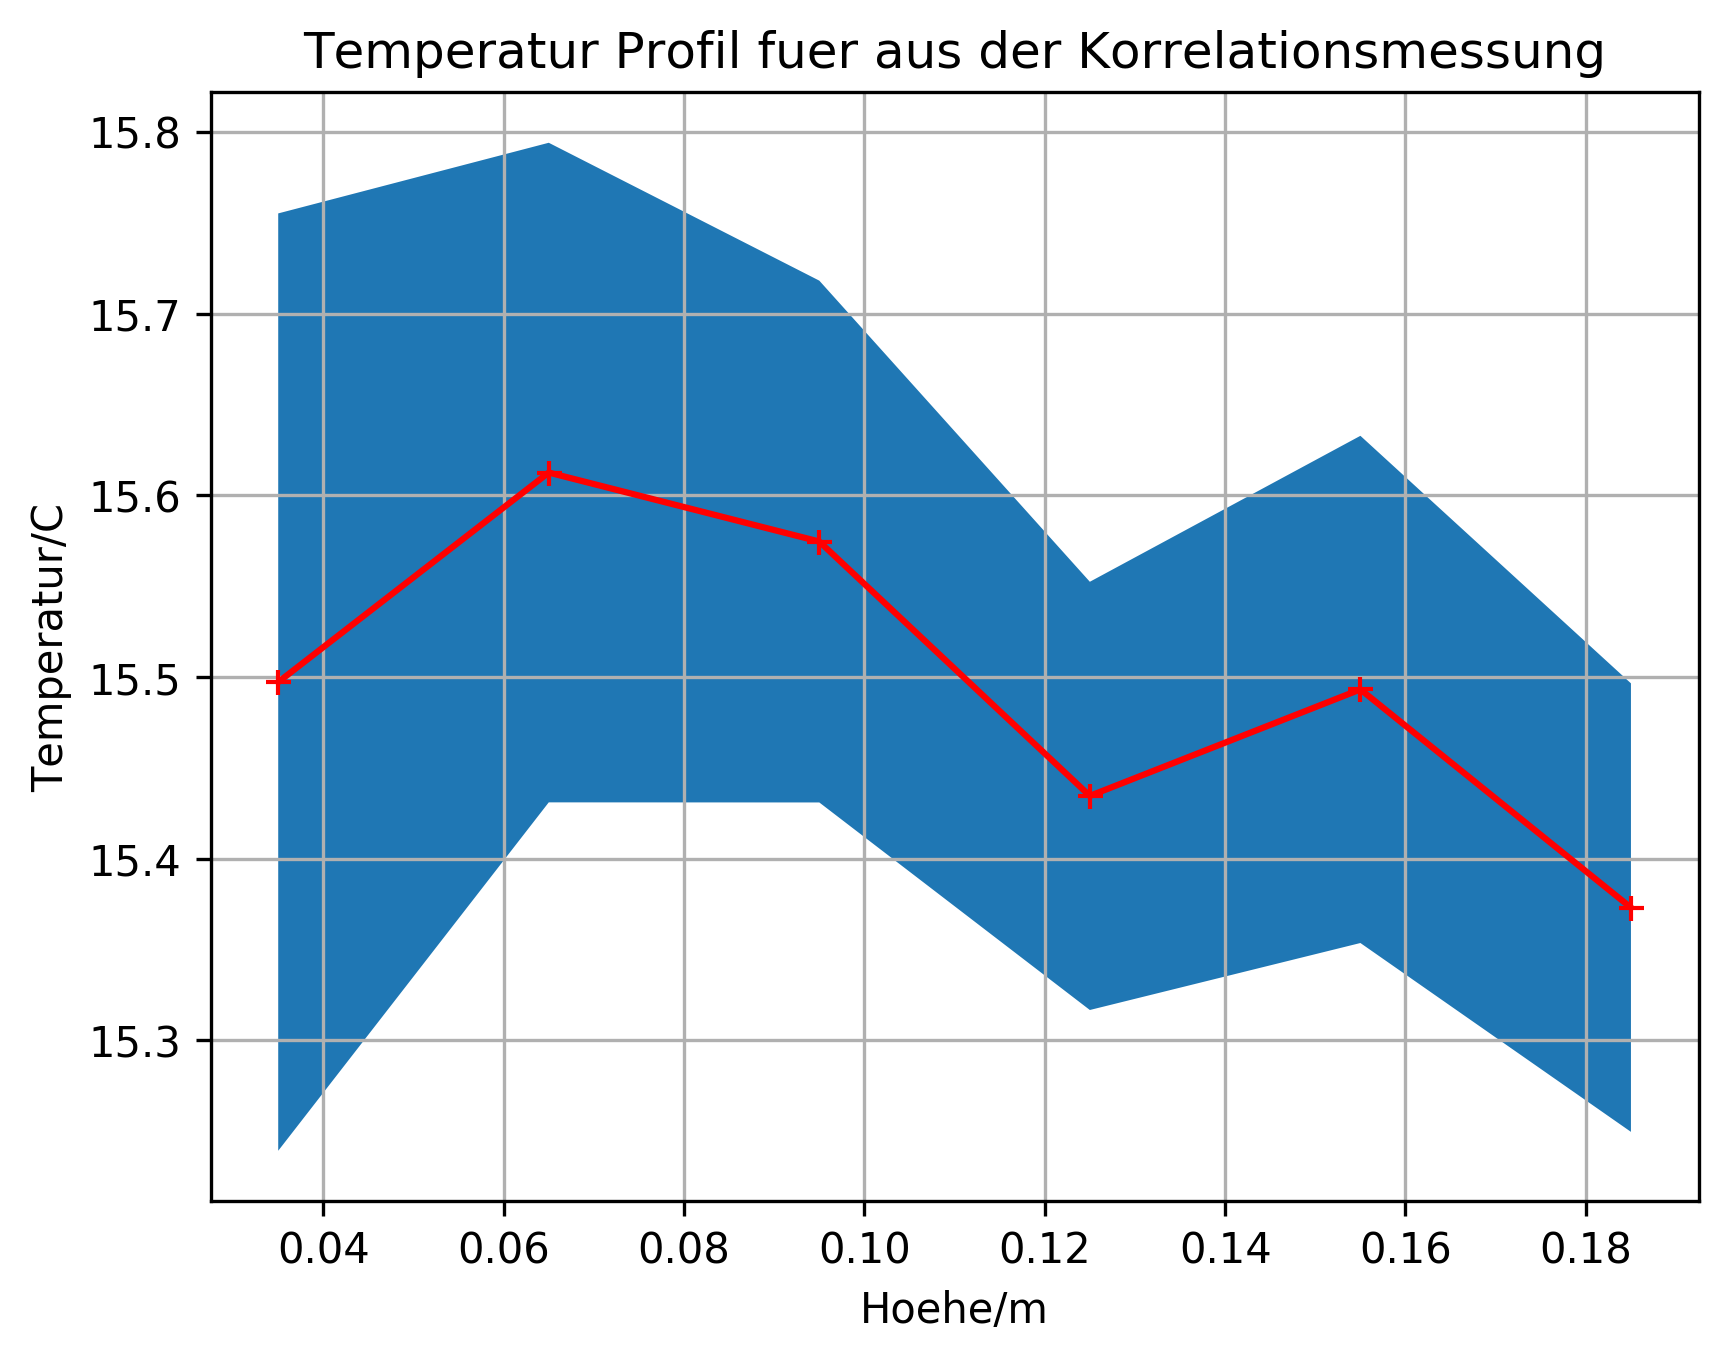
\includegraphics[width=0.8\textwidth]{T_kor.png}
\caption{Temperatur aus der Korrelationsmessung}
\label{fig:T_kor}
\end{figure}





\subsection{Vergleiche der Geschwindigkeiten}

\subsection{Nusselt-Zahl}

\begin{figure}[!ht]
\centering
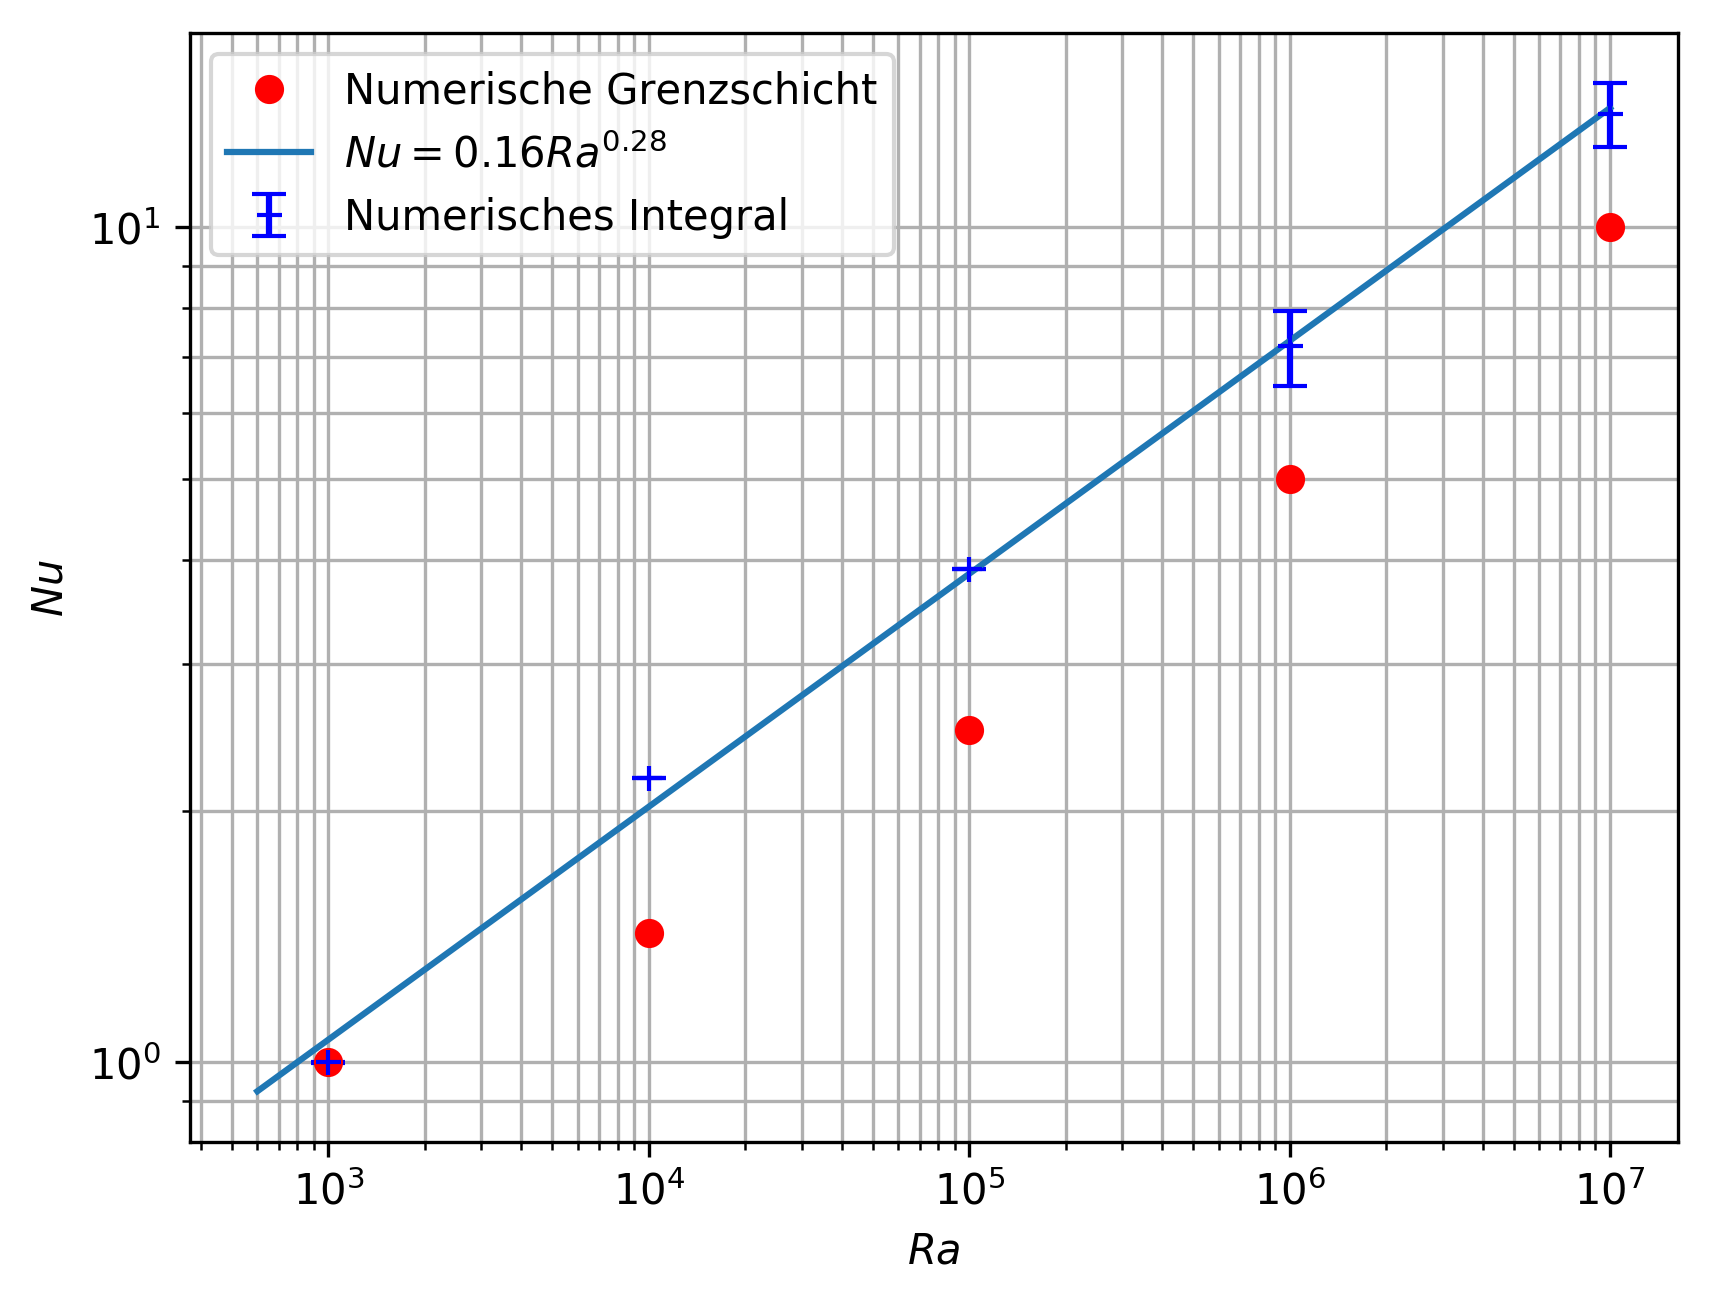
\includegraphics[width=0.8\textwidth]{Nu_Ra.png}
\caption{Nussel Zahl gegen Rayleigh Zahl aufgetragen.}
\label{fig:Nu_Ra}
\end{figure}






\subsection{Temperaturhistogramme}

\begin{figure}[!ht]
\centering
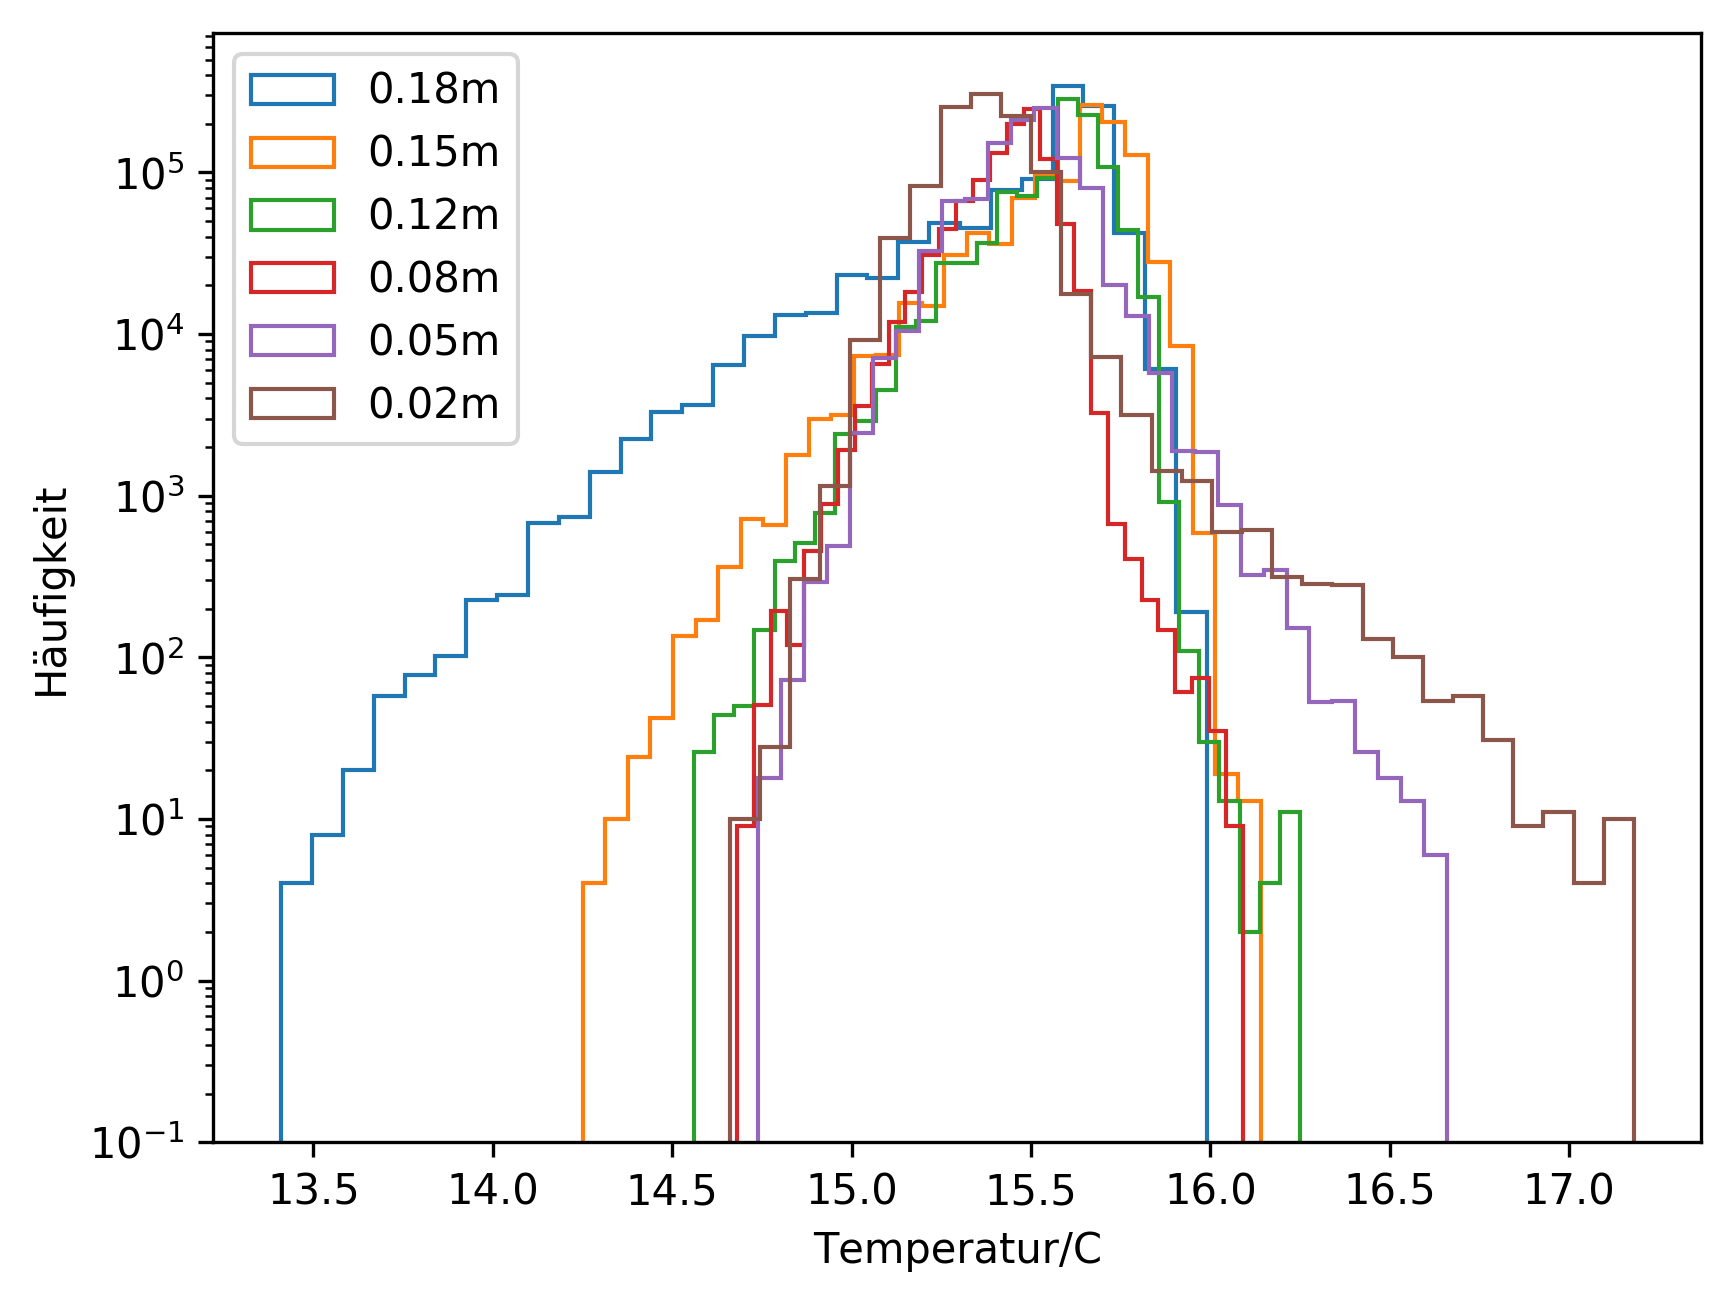
\includegraphics[width=0.8\textwidth]{hist.png}
\caption{Histogram der Temperaturen}
\label{fig:hist}
\end{figure}


\newpage
\section{Bewertung der Ergebnisse}
\label{sec:diskussion}

\newpage
\section{Anhang}
%Zahlen Überarbeiten und runden
\begin{table}
\centering
\begin{tabular}{|l|rrrr|}
\hline
                                            &          Zelle &         Erdkern &      Erdmantel &    Atmosphäre \\
\hline\hline
$\alpha~[\si{\per\kelvin}]$                  &    0.00021     &     1.2e-05     &    1.5e-05     &     0.0037      \\
$\rho~[\si{\kilo\gram\per\cubic\meter}]$     & 1000           & 12000           & 5000           &     1.29        \\
 $c_p~[\si{\joule\per\kilo\gram\per\kelvin}]$ & 4187           &   800           & 1200           &  1000           \\
 $\lambda~[\si{\watt\per\meter\per\kelvin}]$   &    0.6         &    30           &   10           &     0.03        \\
 $\mu~[\si{\pascal\second}]$                  &    0.001       &     0.012       &    1e+21       &     1.7e-05     \\
 $\nu~[\si{\square\meter\per\second}]$        &    1e-06       &     1e-06       &    2e+17       &     1.31783e-05 \\
 $\kappa~[\si{\square\meter\per\second}]$     &    1.43301e-07 &     3.125e-06   &    1.66667e-06 &     2.32558e-05 \\
 $L~[\si{\meter}]$                            &    0.2         &     2.26e+06    &    2.855e+06   & 15000           \\
 $dT~[\si{\kelvin}]$                          &   10           &  2000           & 1000           &    65           \\
 $Pr$                                       &    6.97833     &     0.32        &    1.2e+23     &     0.566667    \\
 $Ra$                                       &    1.15009e+09 &     8.69672e+29 &    1.02731e+07 &     2.59817e+22 \\
\hline
\end{tabular}
\caption{Tabelle der Parameter und wichtige Stoffgrößen}
\label{tab:par}
\end{table}

\newpage
%\nocite{*} %sorgt dafuer, dass alles ausgegeben wird
\printbibliography[heading=bibintoc]
\end{document}
